\documentclass[UTF8]{article}
\usepackage{CJK}
\usepackage{ctex}
\usepackage{color}
\usepackage{pdflscape}
\usepackage{multicol}
\usepackage{amsmath,amssymb,amstext} 
\usepackage{mathrsfs}
\usepackage{float}
\usepackage{cases}           
\usepackage{fancyhdr}        
\usepackage{graphicx}        
\usepackage{tabularx}        
\usepackage{multirow}        
\usepackage{multicol}        
\usepackage{appendix}
\usepackage{geometry}
\geometry{left=2.5cm,right=2.5cm,top=2.5cm,bottom=2.5cm}
\usepackage{mathrsfs}
\usepackage{times}              
\usepackage{amsfonts}           
\usepackage{slashbox}
\usepackage{booktabs}
\usepackage{longtable}
\usepackage{subfigure}

\newcommand{\RNum}[1]{\uppercase\expandafter{\romannumeral #1\relax}}



\newcommand{\enabstractname}{Abstract}
\newcommand{\cnabstractname}{\large[摘要]}
\newenvironment{cnabstract}{%
    \par\small
    \noindent\mbox{}\hfill{\bfseries \cnabstractname}\hfill\mbox{}\par
    \vskip 2.5ex}{\par\vskip 2.5ex}

\begin{document}
\title{“同心协力”策略研究\\
    }

\maketitle
%--------------------------------------------摘要---------------------------------------------
\begin{cnabstract}

\thispagestyle{plain}
本文研究了同心鼓游戏中球与鼓实际碰撞过程的多种情况,建立了非完全弹性碰撞模型、刚体转动模型,使用非线性规划模型
、力矩平衡、刚体力学、最优控制策略、微元法算法进行求解,以对实际游戏策略提出改进方案,模拟结果与现实非常吻合,进行过模型的分析与检验,同时提出了模型的改进策略。\\  

\textbf{对于问题一:}我们将问题一考虑为非完全弹性碰撞的过程分析,及最优化目标求解的问题。球从鼓面40cm处竖直落下,
球被颠起的高度应离开鼓面40cm以上。为消除歧义,此处“离开鼓面”理解为运动过程中球与鼓面的最大距离,
而非球距离碰撞点的距离。最佳协作策略定义为满足该条件时,外力对球做功最少。结合约束条件,使用Lingo求解最优状态。
最终我们给出的最优协作策略是,当八人拉鼓,绳长0.843m时,排球从40cm高处落下,当球落到贴近鼓面时八人瞬时(约0.1s)给出
一个约17.6N的力便不再发力,此时鼓便具有了大小为0.456m/s方向向上的速度,随后立即与球发生碰撞,再次使球弹起至40.9cm自由落下,
而鼓不会上升,然后重复上述过程。\\

\textbf{对于问题二:}
我们将问题二考虑为在不同发力参数下,进行多点受力的刚体的转动过程分析,建立鼓面转动模型并求解的问题,我们利用转动定律、微元
法等公式或思想,建立了合理的模型,并使用Matlab对鼓面倾斜角度进行计算。经计算,八位队员在九组不同发力参数下,鼓面倾斜角
度分别为:0.210°、0.344°、0.148°、0.244°、0.645°、0.282°、1.354°、0.430°、0.135°。\\

\textbf{对于问题三:}本题根据问题二的模型对问题一给出的策略进行修改。鼓面倾斜时,小球后续运动将由竖直上抛转变为斜抛运动。
通过建模计算我们发现,问题二中情况8产生的倾角最大,代入第一问设置的参数(绳长0.843m,鼓面低于绳拉直水平面0.2m),
并认为队员1失误时产生的力是其他队员的$\frac{9}{8}$,取19.8N,
则产生的最大倾角为2.236°,排球可以飞起0.40953592m,满足条件,不用更改力的大小。
根据出错概率,进行人员换位,由(1,2,3,4,5,6,7,8)变为(1,2,3,5,6,4,7,8)并使一直出错的1号同学对面的6号同学力度加大到19.8N。
根据检验,倾角度数有明显减小。\\

\textbf{对于问题四:}
本题是斜抛运动与第二题的鼓面倾角调整结合的最优化策略问题,使得碰撞后排球回归竖直弹跳运动且排球弹起后与鼓面的最大高度差要超过40cm。
分析排球对称斜抛的运动轨迹,精确计算速度,在高度约束条件下计算出碰撞后排球速度的最小值为2.8014m/s,反推出碰撞前鼓的速度为0.171m/s。
以此为据计算出使鼓产生此动量的人均发力为75.4N。再令之部分队员(1、10、3)提前0.1s发力,并加大力度,对鼓的角度进行调整,最终得出每个人的发力大小。
1、10、3号分别沿绳给出的平均的力为54.2N、95.2N、88.1N. 其余人发力均为75.4N(具体站位参见第四题-图15)。\\

\textbf{关键词:微元法\quad 非线性规划模型\quad 力矩平衡\quad 刚体力学\quad 最优控制策略}
\end{cnabstract}

\newpage
\begin{center}
    \section{问题重述}
\end{center}
\subsection{问题背景}
\thispagestyle{plain}
同心鼓是一项考验团队配合协作能力的拓展项目。双面牛皮鼓身中间固定多根长度相同的绳子,在鼓身中部的固定点沿圆周呈均匀分布。
项目开始时,球从保持水平的鼓面中心上方竖直落下,队员同心协力相互配合,仅抓握绳子的末端拉动同心鼓,使球
在鼓面上有节奏地颠起,并使连续颠球的次数尽可能多。
\subsubsection{问题重述}
项目使用双面牛皮鼓颠起排球,开始时,球从鼓面中心上方0.4m处竖直落下,使球被连续颠起的高度应离开鼓面0.4m以上,否则项目停止。
\par\setlength\parindent{2em}
(1)理想状态下,每个人精确控制发力参数,讨论此情形下团队的最佳协作策略,并给出该策略下的颠球高度。
\par\setlength\parindent{2em}(2)现实情形中,队员发力参数很难精确控制,由于误差,鼓面可能出现倾斜。
试建立模型描述队员的发力时机和力度与某一特定时刻的鼓面倾斜角度的关系,并求0.1 s时鼓面的倾斜角度。 
\par\setlength\parindent{2em}(3)现实情形中,根据问题2的模型,讨论在问题1中给出的策略是否需要调整并给出相应策略。
\par\setlength\parindent{2em}(4)鼓面倾斜时,球跳动方向不再竖直,需要队员调整拉绳策略,将球调整为竖直状态弹跳,
计算在精确控制条件下所有十名队员的发力时机及力度,并分析在现实情形中这种调整策略的实施效果。\\ 

\begin{center}
     \section{模型假设}  
\end{center} 

\par\setlength\parindent{2em}
假设 1:经公式计算,空气静止时排球所受的风阻约为排球所受重力的$\frac{1}{30}$,故此处忽略风阻不计。 

假设 2:假设鼓面与排球发生碰撞时,人不对绳发力,系统不受外力影响。

假设 3:假设队员可在瞬时(0.1s)给鼓以一定的动量

假设 4:当鼓面与水平倾角小于3°时,我们都认为鼓与排球发生了对心碰撞,满足动量守恒。

假设 5:假设队员绕鼓均匀分布,力水平投影过圆心。

假设 6:假设鼓皮绷得足够紧,不考虑鼓的形变,视鼓为拥有全表面的薄壳圆柱刚体。\\

\begin{center}
    \section{符号说明}   
\end{center}

\begin{center}
    \begin{table}[h]
        \centering
        \begin{tabular}{p{3cm}<{\centering}|p{7cm}<{\centering}} %设置了每一列的宽度,强制转换。  
            \toprule 
            符号&意义\\
            \hline
            e&PVC材料(皮革类似物)的恢复系数\\
            \hline
            $m_1$&鼓的质量\\
            \hline
            $h_1$&第一阶段鼓上升的高度\\
            \hline
            $v_1$&第一阶段结束(碰撞前)鼓的速度\\
            \hline
            $m_2$&排球的质量\\
            \hline
            $h_2$&第一阶段排球下降的高度\\
            \hline
            $v_2$&第一阶段结束(碰撞前)排球的速度\\
            \bottomrule 
        \end{tabular}  
    \end{table}  
\end{center}
\begin{center}
    \begin{table}[h]
        \centering
        \begin{tabular}{p{3cm}<{\centering}|p{7cm}<{\centering}} %设置了每一列的宽度,强制转换。  
            \toprule 
            符号&意义\\
            \hline
            $v_1^{\mbox{'}}$&碰撞后鼓的速度\\
  
            \hline
            $v_2^{\mbox{'}}$&碰撞后排球的速度\\
            \hline  
            $g$&重力加速度(9.81$m/s^2$)\\
            \hline
            $t_1$&碰撞后排球到达最高点所需时间\\
            \hline
            $t_2$&碰撞后鼓下落到最低点所需总时间\\
            \hline
            $t_{21}$&碰撞后鼓上升阶段所需时间\\
            \hline
            $t_{22}$&碰撞后鼓下落阶段所需时间\\
            \hline
            $x_1$&碰撞后鼓上升阶段经历的路程\\
            \hline
            $W_{\mbox{外}}$&鼓所受外力总功\\
            \hline
            $I_1$&鼓瞬时接受的冲量\\
            \hline
            $F_{\mbox{合竖直}}$&鼓所受的竖直合外力\\
            \hline
            $t_{\mbox{瞬}}$&队员瞬时发力的时间\\
            \hline
            $P_1$&鼓瞬时获得的动量\\
            \hline
            $\theta$&绳拉力与水平面所成角度\\
            \hline
            $T$&绳子的拉力\\
            \hline
            $T_{\mbox{竖直}}$&绳子拉力的竖直分量\\
            \hline
            $T_{\mbox{水平}}$&绳子拉力的水平分量\\
            \hline
            $v_{\mbox{合}}$&排球斜抛合速度\\
            \hline
            $v_{\mbox{竖直}}$&排球斜抛合速度的垂直分量\\
            \hline
            $v_{\mbox{水平}}$&排球斜抛合速度的水平分量\\
            \hline
            $x_{\mbox{水平}}$&斜抛运动的水平位移\\
            \hline
            $J$&转动惯量\\
            \hline
            $\overrightarrow{\beta}$&刚体定轴转动角加速度\\
            \hline
            $\overrightarrow{\omega}$&刚体定轴转动角速度\\
            \hline
            $\overrightarrow{\alpha}$&刚体定轴转动弧度\\
            \hline
            $\overrightarrow{R_i},i=1,2···,8$&各人手相对原点的位矢\\
            \hline
            $\overrightarrow{r_i},i=1,2···,8$&鼓边各点相对原点初始静止时的位矢\\
            \hline
            $\overrightarrow{l_i},i=1,2···,8$&鼓边各点相对原点的位矢\\
 
            \hline
            $\overrightarrow{F_i},i=1,2···,8$&每个人对绳的拉力\\
            \hline
            $\overrightarrow{F}$&绳子对鼓的合力\\
            \bottomrule 
        \end{tabular}  
    \end{table}  
\end{center}
\begin{center}
    \begin{table}[h]
        \centering
        \begin{tabular}{p{3cm}<{\centering}|p{7cm}<{\centering}} %设置了每一列的宽度,强制转换。  
            \toprule 
            符号&意义\\
            \hline
            $\overrightarrow{l_i},i=1,2···,8$&鼓边各点相对原点的位矢\\
            \hline
            $\overrightarrow{M_i},i=1,2···,8$&每根绳上的分力矩\\
            \hline
            $\overrightarrow{M}$&合力矩\\
            \hline
            $R$&鼓面半径\\
            \hline
            $h$&鼓身高度\\ 
            \bottomrule 
        \end{tabular}  
    \end{table}  
\end{center}



\begin{center}
    \section{问题一:非完全弹性碰撞的过程求解}  
\end{center}


\subsection{问题分析与模型建立}
首先对本题的运动学过程进行分析:
根据题设要求项目开始时,球从鼓面40cm处竖直落下,球被颠起的高度应离开鼓面40cm以上。为消除歧义,此处“离开
鼓面”理解为运动过程中球与鼓面的最大距离,而非球距离碰撞点的距离。最佳协作策略定义为满足该条件时,外力对球做功最少。
运动分析如下图所示:
\begin{center}
    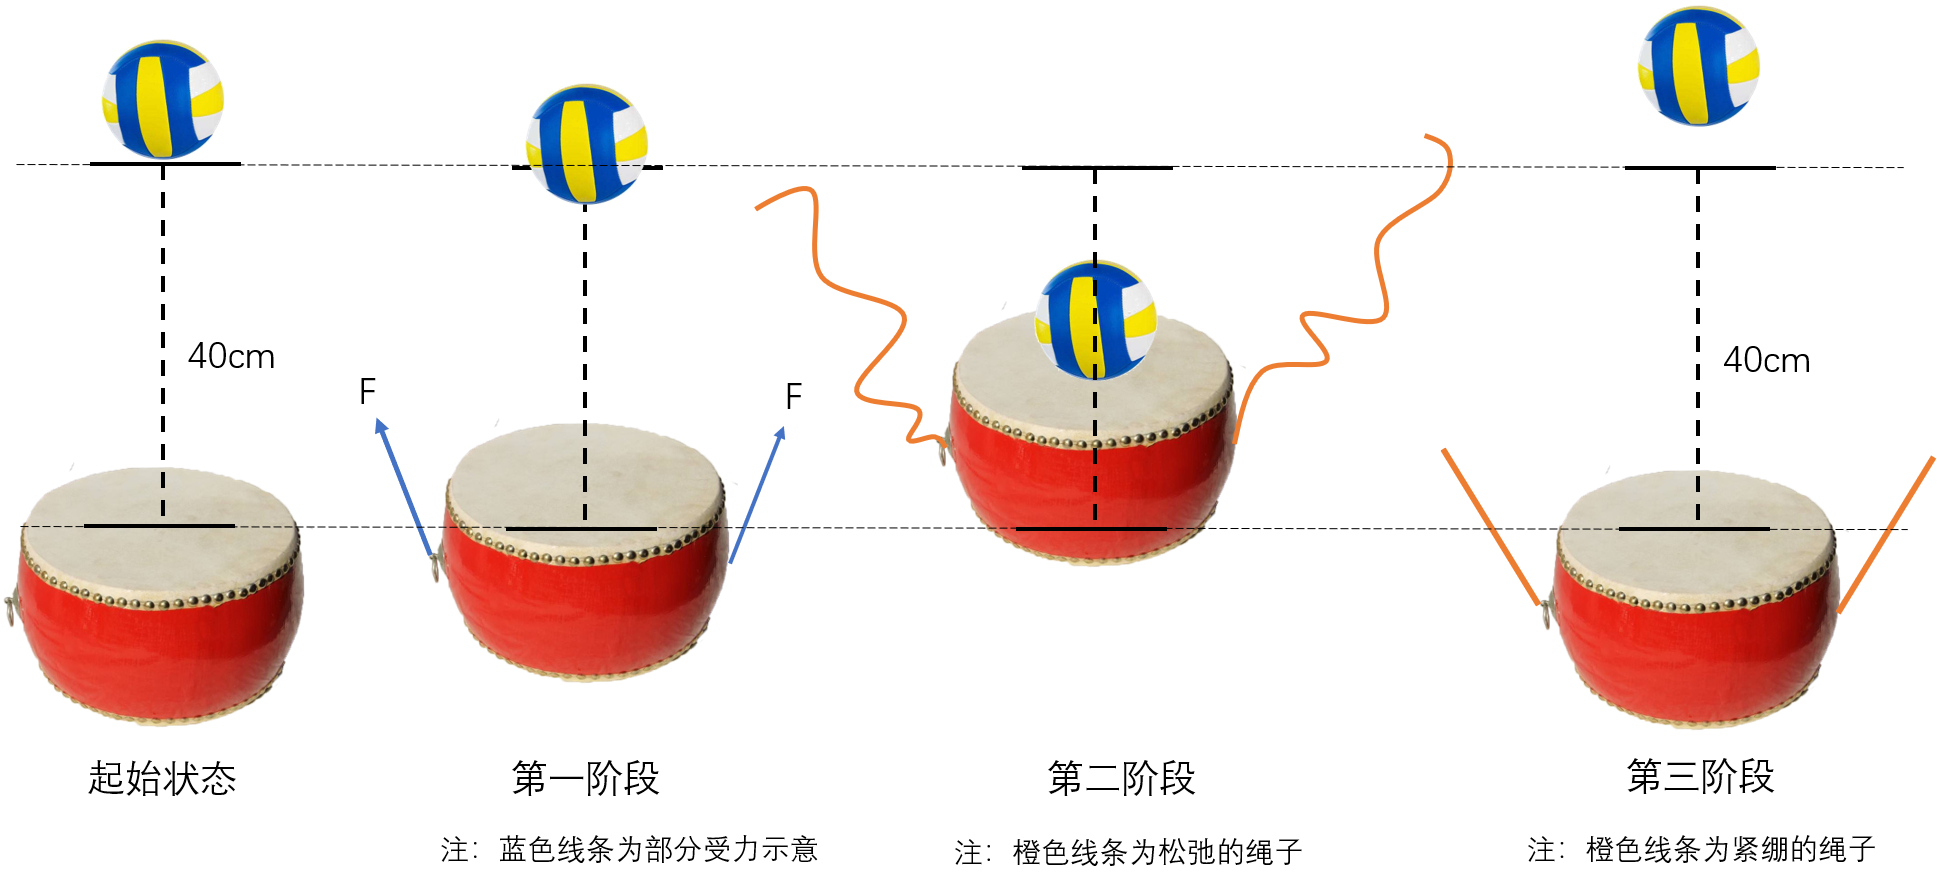
\includegraphics[width=0.95\textwidth]{figure1.png}\\ 
    图1:排球与鼓面相撞的运动过程分析  
\end{center}

排球下落与鼓面相碰并反弹这一运动过程,我们分为三个阶段进行分析:

第一阶段:由拉鼓的同学共同发力,水平作用力相互抵消,竖直作用力为排球提供向上运动的拉力。而排球则在此时做自由落体运动。
经计算,空气静止时排球所受的风阻约为排球所受重力的$\frac{1}{30}$,故此处忽略风阻不计。

第二阶段:在空中的某一位置,排球与鼓面发生碰撞,此时人已撤出外力,则全系统动量守恒。但因为物体材料原因,发生的碰撞
为非完全弹性碰撞。查询维基百科提供的资料[1]可知皮革类似物PVC的恢复系数e=0.86,以此为据进行接下来的计算。

第三阶段:碰撞后鼓的状态为上升或下降(需由计算确定),排球上升,二者达到最大高度差时应大于40cm。在此约束条件下,我们希望
外力对鼓所做的功最小,即是我们对最佳协作策略的判断标准。

\subsection{问题的求解}
\subsubsection{第一阶段}
鼓的质量为$m_1$,第一阶段鼓上升的高度为$h_1$($m$),直到第二阶段碰撞前鼓已经加速到$v_1$

排球的质量为$m_2$,第一阶段排球下降的高度为$h_2$($m$),直到第二阶段碰撞前排球已经加速到$v_2$.根据能量守恒定律[2]有:
\begin{equation}
    \begin{cases}
        h_1+h_2=0.4\\
        \frac{1}{2}m_2v_2^2=m_2gh_2
    \end{cases}
\end{equation}
规定向上为正方向,我们不难理解,$v_1$为正,$v_2$为负。因此
\begin{equation}
    v_2=-\sqrt{2gh_2}
\end{equation}

\subsubsection{第二阶段}
鼓以速度$v_1$和速度为$v_2$的排球发生碰撞。碰撞发生后,鼓的速度变为$v_1^{\mbox{'}}$,排球的速度变为$v_2{\mbox{'}}$',
根据动量守恒[3],恢复系数定义[4],题干条件,列出以下表达式:

\begin{equation}
    \begin{cases}
        m_1v_1+m_2v_2=m_1v_1^{\mbox{'}}+m_2v_2^{\mbox{'}}\\
        e=\frac{v_2^{\mbox{'}}-v_1^{\mbox{'}}}{v_1-v_2}\\
        m_1=3.6,m_2=0.27,e=0.86
    \end{cases}
\end{equation}
根据碰撞问题的能量分析[4],我们得到
\begin{equation}
    \begin{cases}
        v_1^{\mbox{'}}=v_1-(1+e)(v_1-v_2)\frac{m_2}{m_1+m_2}\\
        v_2^{\mbox{'}}=v_2+(1+e)(v_1-v_2)\frac{m_1}{m_1+m_2}
    \end{cases}
\end{equation}

\subsubsection{第三阶段}
鼓开始进行竖直上抛或自由落体或竖直下抛中的一种运动,而小球则进行向上的竖直上抛运动。因为鼓落到最低点会被绳拽住,不考虑绳的形变则鼓的速度
在极短时间内骤减为0,则鼓的下落最大位移为$h_1$那么,排球至少要产生$h_2$的位移,即回到原点才能达到距离差40cm的条件。

根据能量守恒定律[2]及正方向的定义有:
\begin{equation}
    \frac{1}{2}m_2v_2^{\mbox{'2}}=m_2gh_2
\end{equation}
因而解得$v_2^{\mbox{'}}\ge-v_2$

将$v_2^{\mbox{'}}\ge-v_2$代入$v_2^{\mbox{'}}=v_2+(1+e)(v_1-v_2)\frac{m_1}{m_1+m_2}$
解得$v_1\ge-0.1559139785v_2$

将$v_1\ge-0.1559139785v_2$代入$v_1^{\mbox{'}}=v_1-(1+e)(v_1-v_2)\frac{m_2}{m_1+m_2}$
解得$v_1^{\mbox{'}}\ge-0.00591397849983996v_2$

因此$v_1^{\mbox{'}}>0$所以鼓所做的是竖直上抛运动

故而产生了短暂的“追逐”过程,即“鼓追球”,为保证40cm的条件则要求,则要求排球到达最高点时,鼓已经到达最低点。因此列出如下约束方程

其中$t_1$为排球到达最高点所需的时间,$t_2$为鼓到达最低点所需总时间,$t_{21}$为鼓竖直上抛上升阶段所需的时间,$t_{22}$为鼓竖直上抛下落阶段
所需的时间,有关系式$t_2=t_{21}+t{22}$。$x_1$表示鼓竖直上抛上升阶段所经历的位移。
\begin{equation}
    \begin{cases}
        gt_1=v_2^{\mbox{'}}\\
        gt_{21}=v_1^{\mbox{'}}\\
        \frac{1}{2}gt^2_{21}=x_1\\
        \frac{1}{2}gt^2_{22}=x_1+h_2\\
        t_2=t_{21}+t_{22}\\
        t_1\ge t_2
    \end{cases}
\end{equation}

解得:
\begin{equation}
    v_2^{\mbox{'2}}-2v_2^{\mbox{'}}v_1^{\mbox{'}}-2h_2g \ge 0
\end{equation}

\subsubsection{求解最优策略}
根据我们设定的初始判断标准,接下来即是要根据约束条件求解min{$W_{\mbox{外}}\frac{1}{2}m_1v_1^2+m_1gh_1$}

使用Lingo(Linear Interactive and General Optimizer)求解最优化解,将如下方程组输入Lingo进行计算
\begin{center}
    $min \{ {W_{\mbox{外}}\frac{1}{2}m_1v_1^2+m_1gh_1} \}$    
\end{center}
\begin{equation}
    \begin{cases}
        h_1+h_2=0.4\\
        v_2=-\sqrt{2gh_2}\\
        v_1^{\mbox{'}}=v_1-(1+e)(v_1-v_2)\frac{m_2}{m_1+m_2}\\
        v_2^{\mbox{'}}=v_2+(1+e)(v_1-v_2)\frac{m_1}{m_1+m_2}\\
        v_2^{\mbox{'}}\ge-v_2\\
        v_2^{\mbox{'2}}-2v_2^{\mbox{'}}v_1^{\mbox{'}}-2h_2g \ge 0\\
        g=9.81; e=0.86; \\
        m1=3.6; m2=0.27;\\
    \end{cases}
\end{equation}

计算得出的结果如下图所示:
\begin{center}
    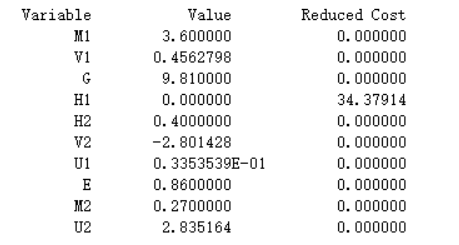
\includegraphics[width=0.5\textwidth]{figure2.png}\\ 
    图2:Lingo计算做功最优解  
    
    注解:图中u1,u2即是$v_1^{\mbox{'}}$,$v_2^{\mbox{'}}$.换名是程序表达的需要
\end{center}

由图我们可以得到$v_1=0.4562798m/s,v_2^{\mbox{'}}=2.835164$

又因为$h_1=0$,故理解为鼓是在瞬时获得的速度,鼓需要获得的瞬时冲量,此处我们取瞬时为0.1s
\begin{equation}
    I_1=(F_{\mbox{合竖直}}-m_1g)t_{\mbox{瞬}}=P_1=m_1v_1
\end{equation}
解得$I_1$=1.64260728‬(N·s)

再假设绳长L,鼓面初始低于人手水平面20cm,则绳端距离人手水平面33cm,对一条绳上所受外力做受力分析如图所示:

\begin{center}
    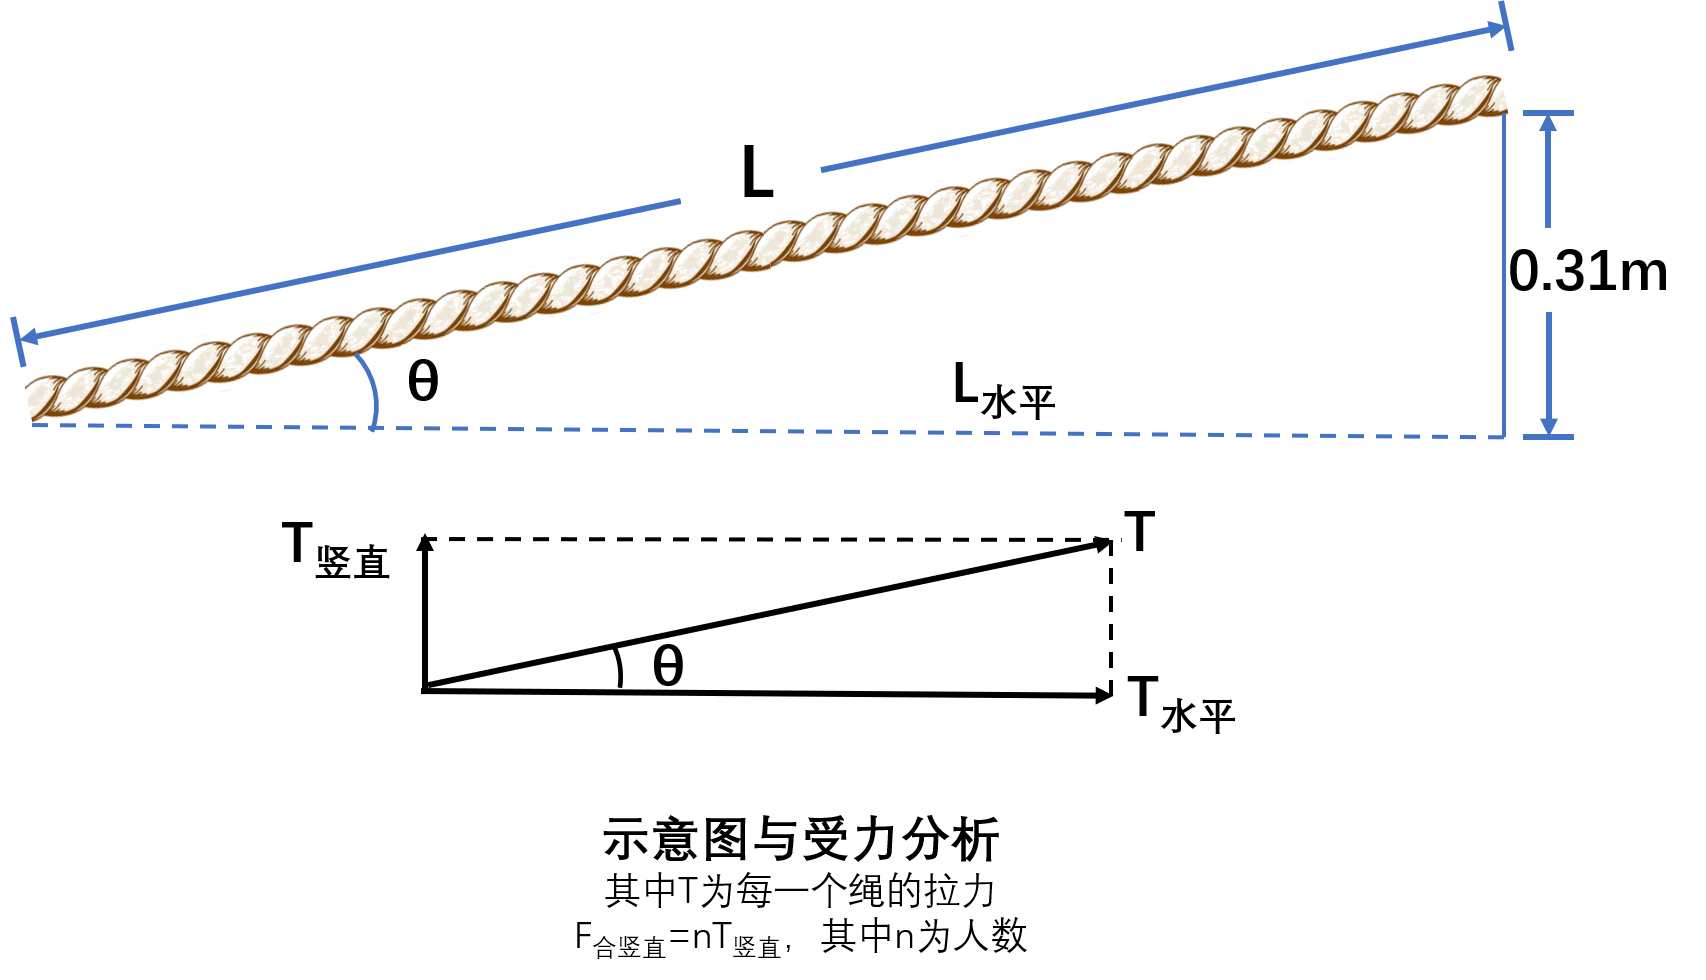
\includegraphics[width=0.6\textwidth]{figure3.png}\\ 
    图3:单条绳的受力分析  
\end{center}

在此情况下假设有8人拉鼓,则
\begin{equation}
    \begin{cases}
        I_1=(F_{\mbox{合竖直}}-m_1g)t_{\mbox{瞬}}\\
        t_{\mbox{瞬}}=0.1\\
        F_{\mbox{合竖直}}=8T_{\mbox{竖直}}\\
        T_{\mbox{竖直}}=sin\theta T\\
    \end{cases}
\end{equation}

可见sin$\theta$的值越大,人所需发力T就越小,也即绳长越短发力越小。根据队员之间的最小距离不得小于60 cm做出如下示意图:
\begin{center}
    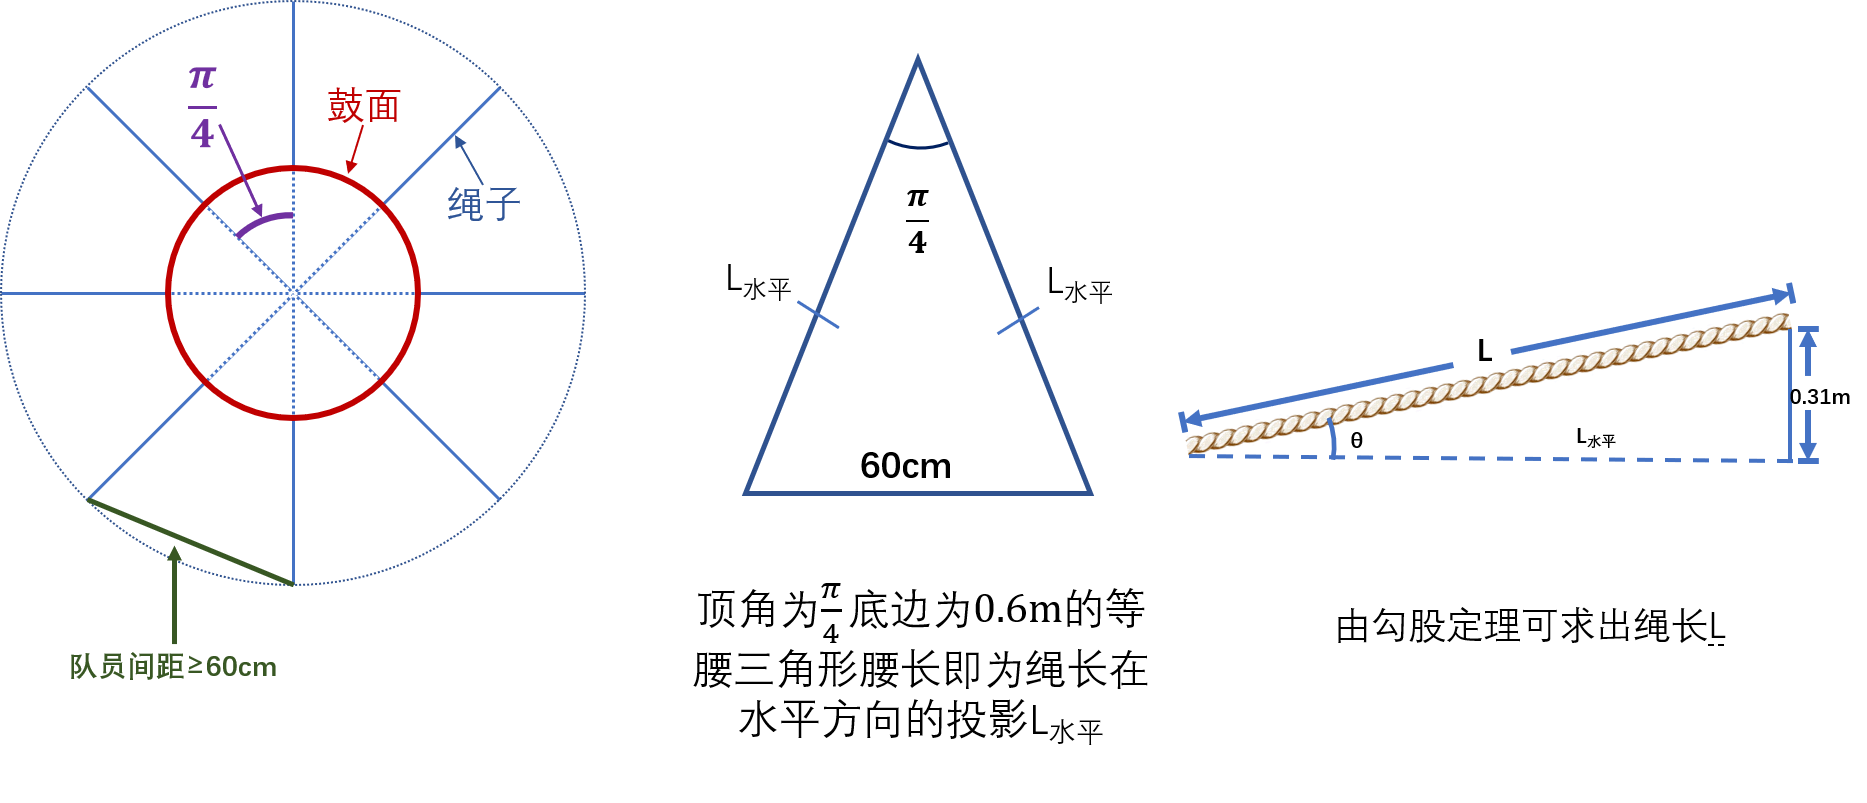
\includegraphics[width=0.95\textwidth]{figure4.png}\\ 
    图4:绳长分析  
\end{center}
根据正弦定理可求得绳长在水平面的投影为$0.3\sqrt{4+2\sqrt{2}}$

再根据勾股定理解得绳长约为0.843m,$sin\theta$=0.367732

在此基础上解得T=17.58776‬N,再根据运动学规律求得排球上升距离为40.969cm.
撞击后鼓的速度为0.033535m/s,上升距离小于1mm可忽略不计

\subsection{最优协作策略}
综上所述,我们给出的最优协作策略是,当八人拉鼓,绳长最短为0.85m时,排球从40cm高处落下,当球落到贴近鼓面时八人瞬时(约0.1s)给出
一个约16.7N的力便不再发力,此时鼓便具有了大小为0.456m/s方向向上的速度,随后立即与球发生碰撞,再次使球弹起至40.9cm自由落下,
而鼓不会上升,然后重复上述过程。

\subsection{模型结果的分析}
对于$W_{\mbox{外}}=\frac{1}{2}m_1v_1^2+m_1gh_1$
根据上述约束条件与$h_1$和$h_2$之间的关系,我们求解得到
\begin{equation}
    \frac{1}{2}m_1v_1^2+m_1gh_1=\frac{1}{2}m_1v_1^2+0.4m_1g-\frac{1}{2}m_1v_2^2
\end{equation}
则现在需要$v_1$尽可能小$v_2$尽可能大。通过$v_2^{\mbox{'}}\ge-v_2$与$v_2^{\mbox{'}}=v_2+(1+e)(v_1-v_2)\frac{m_1}{m_1+m_2}$可得上式关系为
\begin{equation}
    W_{\mbox{外}}=\frac{1}{2}m_1v_1^2+0.4m_1g-\frac{1}{2}m_2v_2^2\ge0.4m_1g-\frac{1}{2}m_1(0.975690831309978)v_2^2
\end{equation}
故而取$v_2$绝对值最大即可。也即$h_2$最大即可。$h_2=0.4$根据约束调节,代入求解得到
$v_1=0.4562798m/s$故而才有了上述结果的产生。

\begin{center}
    \section{问题二:发力参数对鼓面倾角的影响}
\end{center}


\subsection{问题分析与模型建立}
对问题二进行分析:
由于问题一为理想状态,而在现实情形中,队员的发力时机和力度很难做到精确控制,故会存在一定误差。当队员人数为8时,初始
时刻鼓面水平静止在较绳子水平以下11cm,存在队员发力大小差异或者发力较早,故实际中鼓面会有一定倾斜。

以鼓质心为坐标原点,鼓面竖直向上,以z轴为转轴,建立如图5所示坐标系:
\begin{center}
    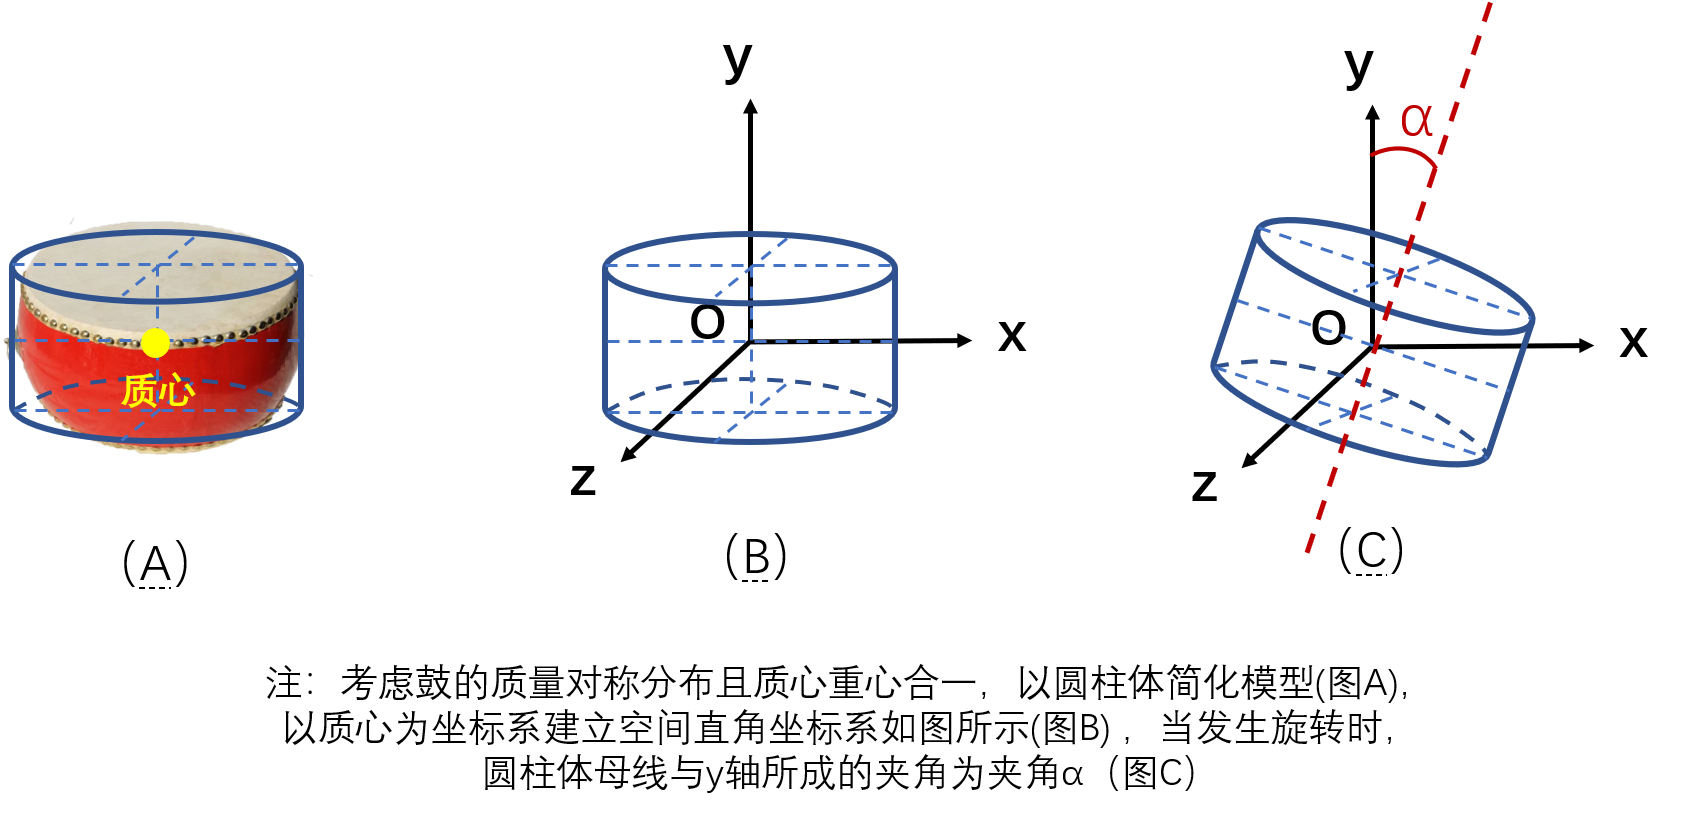
\includegraphics[width=0.95\textwidth]{figure5.png}\\
    图5:鼓模型静止及偏转时坐标系建立
\end{center}

因为本题中,受力点位于鼓侧,且存在不同时间,不同发力状态的情况。考虑到当发力状态不对称时,转动的形式将极为复杂,所以建
系时,我们通过调整坐标系,使得发力状态关于xoy平面对称,转轴与z轴平行。
假设鼓皮紧绷,鼓形变可以忽略,鼓可视作刚体,且队员发力后,一直维持该力到0.1s时刻。

设物体质量为m,$m=\int_{m}\, dm$,设r为质点dm到转轴的垂直距离,对于连续的质点系,则转动惯量为J,转动惯量计算公式[5]为$J=\int_{m} r^2\, dm$

根据力矩的计算公式[6],设$\overrightarrow{F}$为施加的作用力,从转轴到施力点的位移矢量为$\overrightarrow{l}$ ,故可得
出力矩$\overrightarrow{M}=\overrightarrow{l}\times\overrightarrow{F}$,力矩方向服从右手螺旋定则[8],由于为矢量,故分力矩可叠加成合力矩

设刚体定轴转动角加速度为$\overrightarrow{\beta}$,再由转动定律[7]可得$\overrightarrow{M}=J\overrightarrow{\beta}$\\
由已求得的角加速度$\overrightarrow{\beta}$,设角速度为$\overrightarrow{\omega}$,可求得0.1s时转动的弧度$\overrightarrow{\alpha}$, 由角
加速度计算公式[6] 得$\overrightarrow{\beta}=\frac{\Delta \overrightarrow{\omega}}{\Delta t}=
\frac{\frac{\Delta \overrightarrow{\alpha}}{\Delta t}}{\Delta t}$,故可得出转动
弧度$\overrightarrow{\alpha}=\frac{1}{2}\overrightarrow{\beta} t^2$,转动角度为$180/\pi*\overrightarrow{\alpha}$\\

\subsection{模型的验证}
设$\overrightarrow{R_{i}}\;(i=1,\cdots,8)$为各人手相对原点的位矢;
$\overrightarrow{r_{i}}\;(i=1,\cdots,8)$ 为鼓边各点相对于原点即鼓质心的初始即静止时的位矢,其中$r_{ix}$、
$r_{iy}$、$r_{iz}$ 分别为该位矢沿x、y、z轴的分量的数值;$\overrightarrow{l_{i}}\;(i=1,\cdots,8)$为鼓边各点相对于原点即鼓质心的位矢。
转动角度(即鼓面倾斜角度)为$\alpha$。
$F_{i}(t)\;(i=1,\cdots,8)$表示每个拉力的大小。
设该坐标系中任一向量可表示为
\begin{equation}
\overrightarrow{r}=x\overrightarrow{i}+y\overrightarrow{j}+z\overrightarrow{k}
\end{equation}
$\overrightarrow{i}$,$\overrightarrow{j}$,$\overrightarrow{k}$分别为x,y,z轴单位方向向量。
由于绕z轴转动,向量沿z轴改变量为0。
则有:
\begin{equation}
\overrightarrow{l_{i}}=r_{ix}\cos\alpha\overrightarrow{i}-r_{ix}\sin\alpha\overrightarrow{j}+r_{iz}\overrightarrow{k}
\end{equation}
设每个人对绳子的拉力为
\begin{equation}
\overrightarrow{F_{i}}=F_{i}(t)\frac{(\overrightarrow{R_{i}}-\overrightarrow{r_{i})}}{\left |\overrightarrow{R_{i}}-\overrightarrow{r_{i}}\right|}\;(i=1,\cdots,8)
\end{equation}
由于沿着一根绳子拉力处处相等,故鼓受绳子拉力也为$\overrightarrow{F_{i}}\;(i=1,\cdots,8)$
由于鼓为刚体,可视作拥有全表面的薄壳圆柱体,由题意可得鼓面半径为R=0.2m,鼓身高度为h=0.22m,

鼓其绕z轴的转动惯量为
\begin{equation}
J=\int_{m}r^2\,dm=\frac{m}{12(R+h)}[3R^{2}(R+h)+2h^2(3R+2h)]=0.0832057
\end{equation}
转动角加速度
\begin{equation}
\overrightarrow{\beta}=\frac{d^{2}\overrightarrow{\alpha}}{dt^{2}}
\end{equation}
根据转动定律[7]得
\begin{equation}
J\overrightarrow{\beta}=\sum_{i=1}^{8} \overrightarrow{F_{i}}\times\overrightarrow{l_{i}}
\end{equation}
\subsection{问题二的求解}
\subsubsection{序号1鼓面倾角}
假设此8人绕鼓均匀分布,绳长$x_0=1.7m$,鼓位于绳水平面11cm以下,根据勾股定理得鼓边点到人手垂直距离为$\sqrt{1.7^2-0.11^2}\approx 1.6964$.

在Oxz平面上,以沿x 轴正方形为第一位队员发力方向,发力为$F_{1}(t)=90$N ,人手1到原点位矢:
\begin{equation}
\overrightarrow{R_{1}}=1.8964\overrightarrow{i}+0.11\overrightarrow{j}+0\overrightarrow{k}
\end{equation}
鼓边1点对原点初始位矢为:
\begin{equation}
\overrightarrow{r_{1}}=0.2\overrightarrow{i}+0\overrightarrow{j}+0\overrightarrow{k}
\end{equation}
第一位队员对绳子的拉力为:
\begin{equation}
\overrightarrow{F_{1}}=F_{1}(t)\frac{(\overrightarrow{R_{1}}-\overrightarrow{r_{1}})}{\left |\overrightarrow{R_{1}}-\overrightarrow{r_{1}}\right|}=89.8114\overrightarrow{i}+5.8237\overrightarrow{j}+0\overrightarrow{k}
\end{equation}
鼓边1点相对于原点的位矢为:
\begin{equation}
\overrightarrow{l_{1}}=r_{1x}\cos\alpha\overrightarrow{i}-r_{1x}\sin\alpha\overrightarrow{j}+r_{1z}\overrightarrow{k}\\
=0.2\cos\alpha\overrightarrow{i}-0.2\sin\alpha\overrightarrow{j}+0\overrightarrow{k}
\end{equation}
力矩1为:
\begin{equation}
\overrightarrow{M_1}=\overrightarrow{F_{1}}\times\overrightarrow{l_{1}}
\end{equation}
逆时针旋转45度为第二位队员发力方向,发力为$F_{2}(t)=80$N\\
$\cdots\cdots$\\
逆时针旋转45度之后7次为第八位队员发力,发力为$F_{8}(t)=80$N
\begin{equation}
\overrightarrow{R_{8}}=-\frac{1.8964}{\sqrt{2}}\overrightarrow{i}+\frac{1.8964}{\sqrt{2}}\overrightarrow{j}+0.11\overrightarrow{k}
\end{equation}
鼓边8点对原点初始位矢为
\begin{equation}
\overrightarrow{r_{8}}=-\frac{2}{\sqrt{2}}\overrightarrow{i}+\frac{2}{\sqrt{2}}\overrightarrow{j}+0\overrightarrow{k}
\end{equation}
第八位队员对绳子的拉力为:
\begin{equation}
\overrightarrow{F_{8}}=F_{8}(t)\frac{(\overrightarrow{R_{8}}-\overrightarrow{r_{8}})}{\left|\overrightarrow{R_{8}}-\overrightarrow{r_{8}}\right|}=56.4500\overrightarrow{i}+5.1763\overrightarrow{j}-56.4500\overrightarrow{k}
\end{equation}
鼓边8点相对于原点的位矢为:
\begin{equation}
\overrightarrow{l_{8}}=r_{8x}\cos\alpha\overrightarrow{i}-r_{8x}\sin\alpha\overrightarrow{j}+r_{8z}\overrightarrow{k}\\
=0.1414\cos\alpha\overrightarrow{i}-0.1414\sin\alpha\overrightarrow{j}-0.1414\overrightarrow{k}
\end{equation}
力矩8为:
\begin{equation}
\overrightarrow{M_8}=\overrightarrow{F_{8}}\times\overrightarrow{l_{8}}
\end{equation}
累加力矩得合力矩:
\begin{equation}
\overrightarrow{M}=\overrightarrow{M_1}+\overrightarrow{M_2}+\cdots+\overrightarrow{M_8}
\end{equation}
同时,我们通过受力分析也可以看出,鼓在做变加速运动,所受合力为:
\begin{equation}
\overrightarrow{F}=\overrightarrow{F_1}+\overrightarrow{F_2}+\cdots+\overrightarrow{F_8}
\end{equation}
所以加速度为:
\begin{equation}
\overrightarrow{a}=\frac{\overrightarrow{F}}{m1}+\overrightarrow{g}
\end{equation}
根据转动定律,可知:
\begin{equation}
J\overrightarrow{\alpha}=\overrightarrow{M}
\end{equation}

所以我们可以根据合力矩,计算出此时鼓面的角加速度。但由前式可知,$t_0$时刻的角加速度与$t_0$时刻鼓面已经转动
过的角度有关,故最终角加速度的表达式为常微分方程,为了简化计算,我们利用MATLAB,利用微元法,将时间t分成了1000 份,每份$\Delta t$ 内可视作受力恒定,角加速度恒定。

求得序号1鼓面倾角为0.20992度
\subsubsection{序号2,3鼓面倾角}

根据已有条件进行受力分析,对坐标轴进行调整,使得所有队员发力方向、状态关于Oxy面对称,使得转轴一
定平行于z轴,同时力矩方向,角加速度方向也平行于z轴。计算细节类似序号1情况。
\subsubsection{序号4,5,6,7,8,9鼓面倾角}
此时出现了发力时间不同的情况,故需要分时间段求解。
第一位队员比其他七位早发力0.1s,此时我们认为,其它队员虽未发力,但我们认为,为了维持鼓的状态,队员们需要提供有维持鼓竖直方向受力平衡的力。
\begin{equation}
\sum_{n=1}^8|F_i|sin\theta_1=m_1g
\end{equation}
\begin{equation}
sin\theta_1=\frac{0.11}{1.7}
\end{equation}

联立解得有:
\begin{equation}
|F_i|\approx64.2
\end{equation}

所以我们认为,在-0.1s时,第一位队员以80N的力,沿绳方向发力,其余人,以64.2N的力,沿绳方向发力,直到0时刻,后续求解也沿用此想法。
所以我们对[-0.1,0]与[0,0.1]两个时间段分别进行求解。

根据求解结果,两次不同的旋转都是小量,考虑到小角度是可加量,故我们根据发力状态分析具体情况,将两次角度相加或相减,得到最终结果。

如:序号9,根据受力分析,两次旋转角加速度方向相反,故最终结果为两次旋转角度相减。经分析,本题所有序号最终结果如下:
\begin{center}
    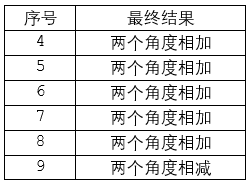
\includegraphics[width=0.25\textwidth]{figure15.png}\\
\end{center}
\subsubsection{求解结果}
利用MATLAB,求解出九组不同发力大小和发力时间对应的鼓面倾角大小,如图6:
\begin{center}
    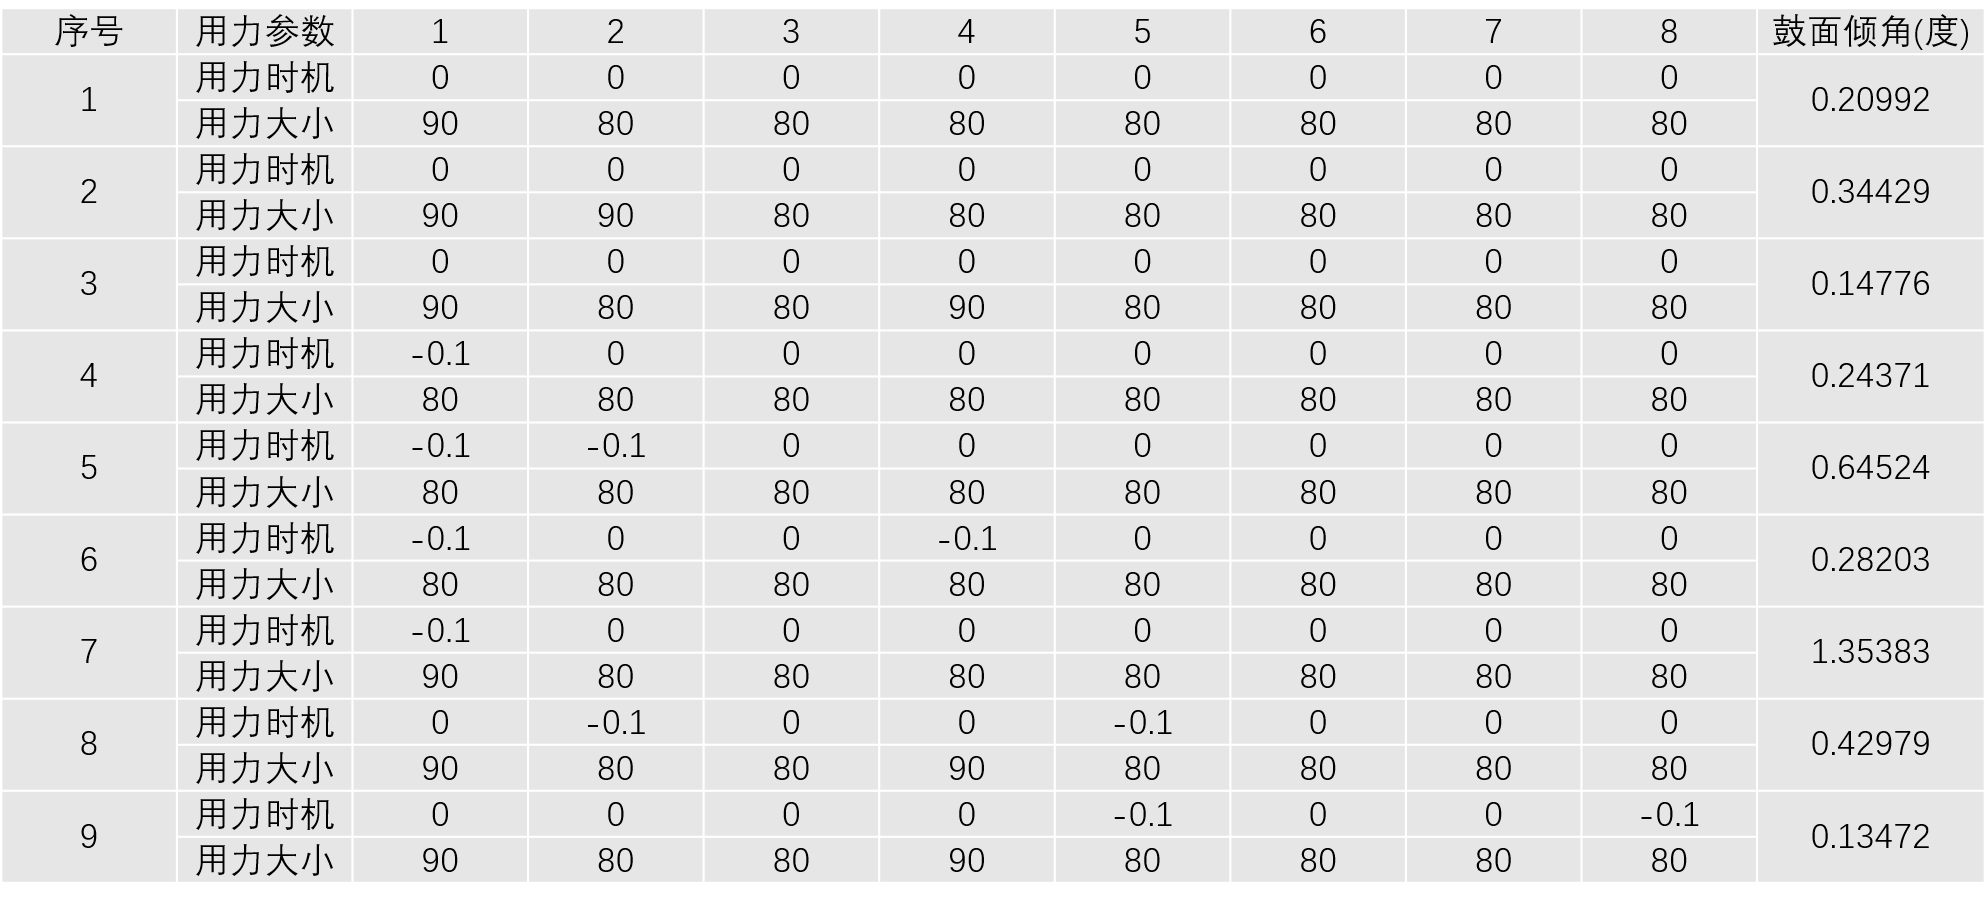
\includegraphics[width=0.95\textwidth]{figure6.png}\\
    图6:发力时机和用力大小对鼓面倾角的影响
\end{center}

\subsection{模型结果的评价}
由计算结果可知,同时作用不同大小的力和有同等大小的力提前作用相比对鼓面倾斜角度影响较小,以题目为例,发力时间
相同时,普通队员发力,特殊力合力越大时,影响鼓面倾斜角度效果越明显,由于普通力与特殊力相差仅10N\~24N左右,且作用
时间仅0.1s,鼓重3.6kg,而且当随着角度增大,特殊力垂直鼓面的分量大小将逐渐减小,普通力垂直鼓面的分量大小将逐渐增大,使
得角加速度逐渐减小,甚至产生反向加速度。所以影响效果总体来说并不明显,倾斜角度小于1 度;若发力时间不同,对鼓倾斜角度影响
略大于题设中发力大小的影响。故为了维持鼓面平衡,从而使颠球次数更多,应尽量使所有队员同时发力。

\begin{center}
    \section{问题三:最大偏角下排球弹起高度的检验及策略调整}  
\end{center}

\subsection{问题分析}
本题是根据问题二的情况对问题一给出的策略进行修改。鼓面由水平变为倾斜后,小球的后续运动也会由竖直上抛转变为斜抛运动。
此时,在碰撞后速度不变的情况下,最大上升高度也会有所下降,我们需要保证,即使不调整鼓面倾角,高度差也要能到达40cm。
而后再对站位策略等进行调整,使得鼓面倾角尽可能减小。\\

\subsection{模型建立}
因为是对第一问进行调整,所以对于第三问的模型,应建立在,人均发力17.6N,绳长为0.843m,鼓面距离绳拉直水平面0.2m的条件下。
当鼓保持不动时受力平衡人均发力为$m_1g/(8sin\theta)=12N$.

根据第二问求解出的表格,我们知道,在第七种情况下,队员1既提前发力又加大发力,倾角最大。若此情况下都可满足高度差大于40cm的条件,则
认为所有情况下都可以满足条件。

\subsection{问题求解}
分析表格易得出,队员发力大小失误总是会比正常发力大约$\frac{1}{8}$,基于此考虑我们认为队员1出现的状况是发力19.8N,提前0.1s发力。
通过第二题的计算方法,得出鼓面倾角应为2.236°

\begin{center}
    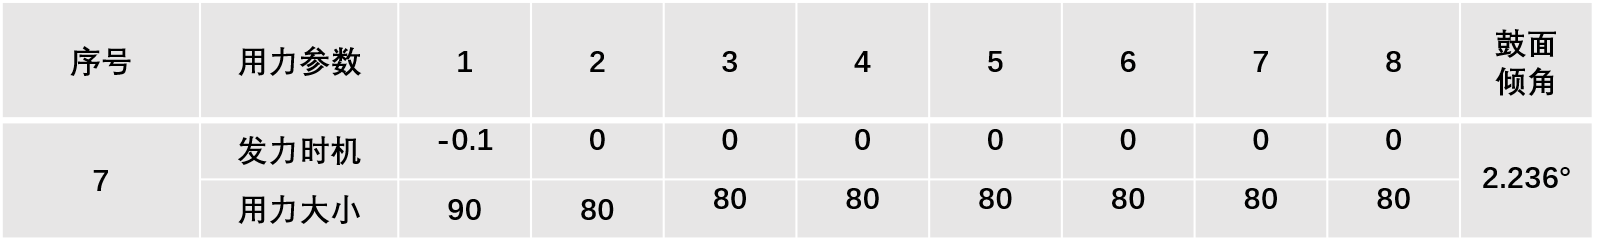
\includegraphics[width=0.95\textwidth]{figure11.png}\\ 
    图7:鼓面倾角分析  
\end{center}

则排球弹起后发生的斜抛与竖直方向所成角度大小应为$2.236°/2=1.118°$,
那么竖直方向的速度就由第一问中的2.835164m/s,变为了$2.835164*cos1.118°=2.8346242747$

那么此时根据$h=\frac{v^2}{2g}$,就可以计算出,此时排球的最大上升高度为0.40953592m,仍旧大于0.4m,满足条件。
所以我们可知即使不对现有情况进行任何调整,排球也能按要求到达目标高度。

但为了使得题目状态最优,我们希望鼓面倾角最小,因此我们对人的站位进行调整。

根据出错情况,我们发现2号同学和4号同学每次出错概率相近,因此让4号同学与5号同学换位,站到2号同学的对面去。同理,
我们发现5号同学和8号同学每次出错概率相近,因此让5号同学与6号换位(原4号位置),站到8号同学的对面去。
站位情况变化如图所示

\begin{center}
    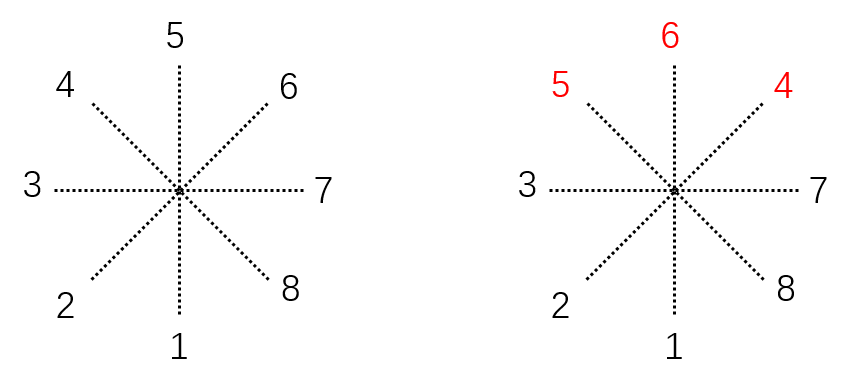
\includegraphics[width=0.5\textwidth]{figure12.png}\\ 
    图8:站位变化情况  
\end{center}

为平衡每次都出错的1号同学,在另从不出错的6号同学每次都多发力$\frac{1}{8}$,即19.8N
以上即为所有的调整情况。

\subsection{模型验证}
为保证我们这样的调整是有效果的。我们对调整前后的倾角大小变化进行了计算,计算结果如下图所示:

\begin{center}
    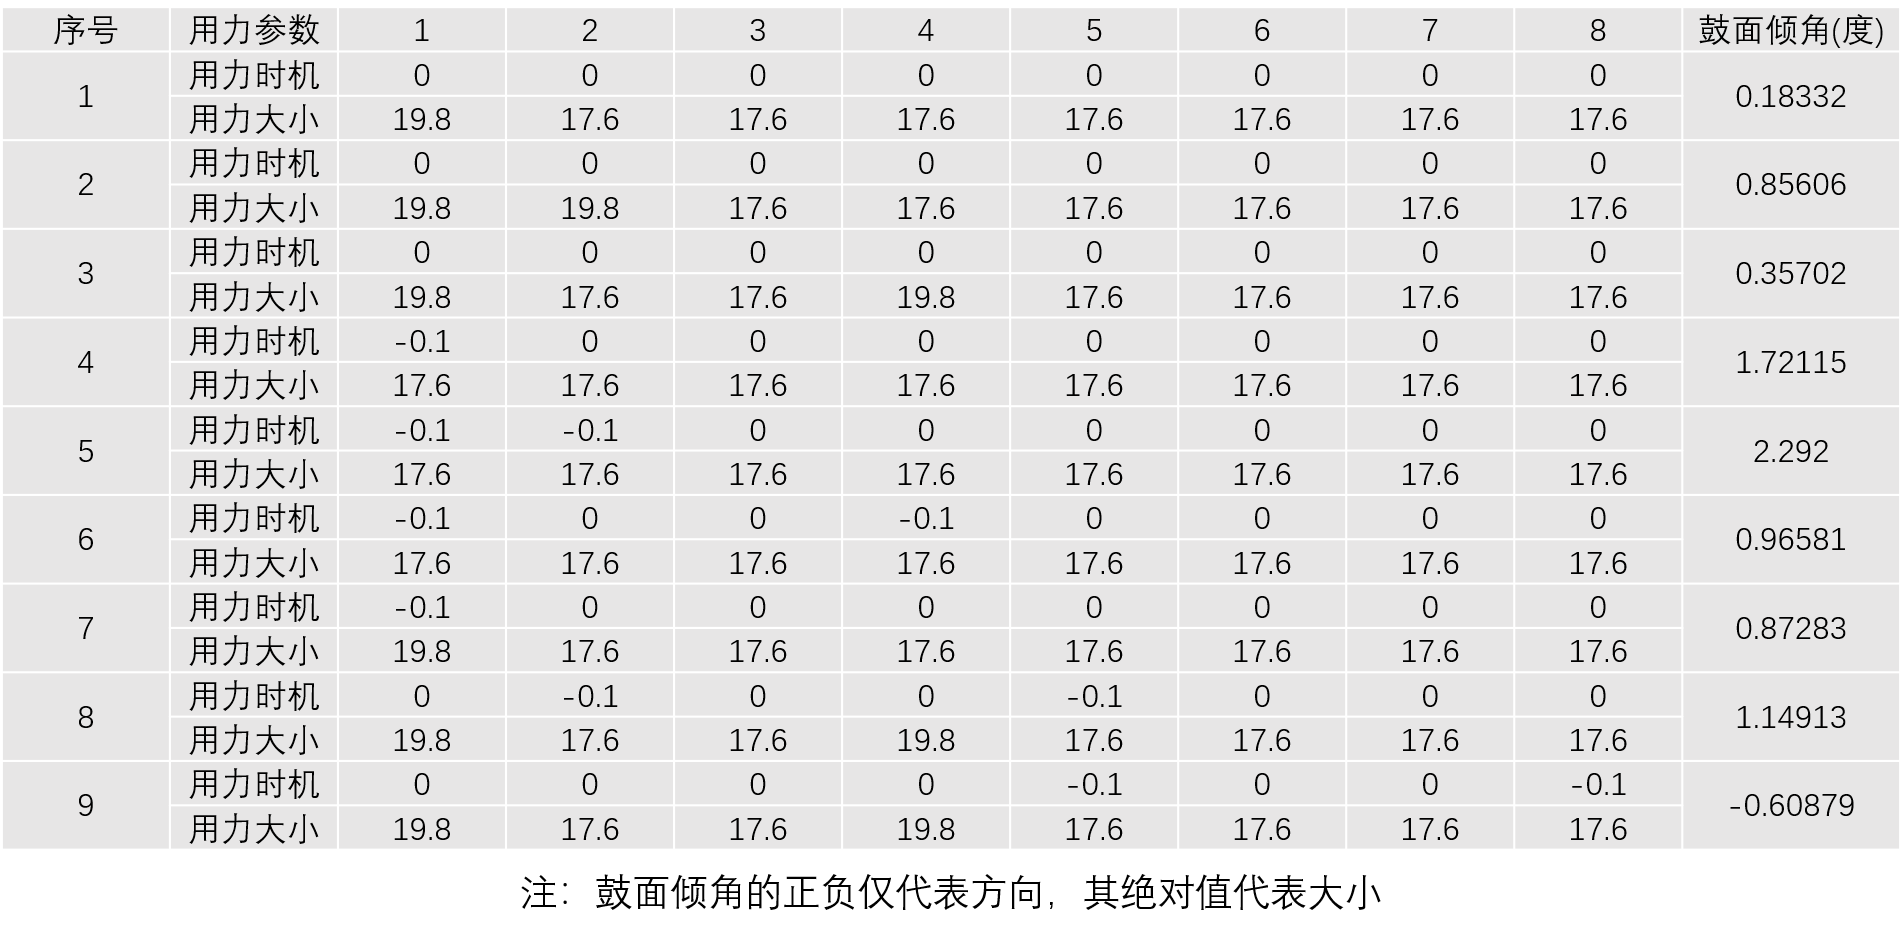
\includegraphics[width=0.95\textwidth]{figure13.png}\\ 
    图9:站位变更前鼓面倾角  
\end{center}

\begin{center}
    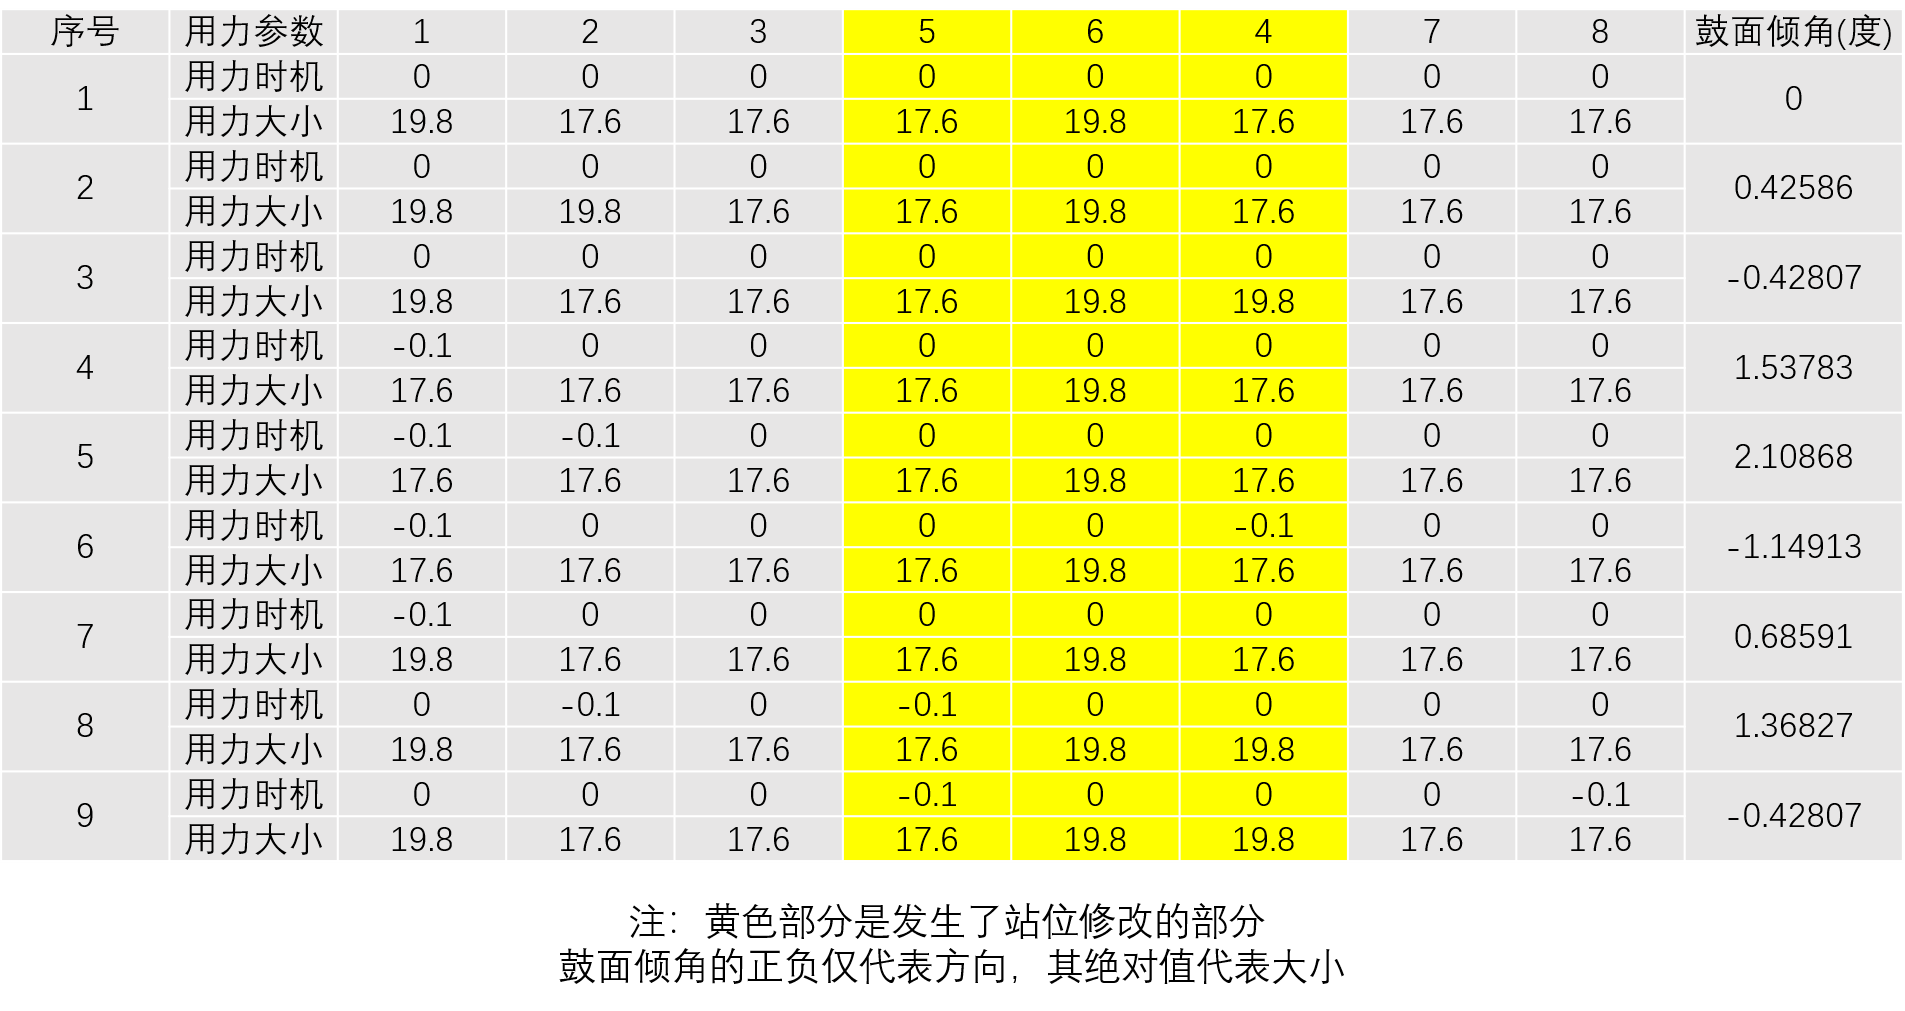
\includegraphics[width=0.95\textwidth]{figure14.png}\\ 
    图10:站位变更后鼓面倾角  
\end{center}

根据结果显示,实验的9次中有6次都产生了角度变小的优势。而角度变大的原因主要是因为失误导致站在对位的(2,4)(5,8)虽然发生的概率相近,
但发生的时机并不完全相同,所以导致了可能会产生倾角变大的情况,但若试验次数较大的情况下,该策略调整是有效的。


\begin{center}
    \section{问题四:斜抛运动与鼓面倾角调整最优化策略}  
\end{center}

\subsection{问题分析}
本题是斜抛运动与第二题的鼓面倾角调整结合的最优化策略问题,力求在较短的时间内,用
较小的力调整鼓面,使得碰撞后排球回归竖直方向的运动且弹起后与鼓面的最大高度差要超过40cm。
我们先分析了排球对称斜抛的运动轨迹,精确计算速度,根据第一问中的碰撞分析(0.5°倾斜的碰撞仍视为正碰)获取碰撞后的速度,
在高度约束条件下计算出碰撞后排球速度的最小值,反推出碰撞前鼓的速度。以此为据计算出使鼓产生此动量的人均发力。再另之前鼓轨迹投影落下的两人
提前发力,加大发力对鼓的角度进行调整,最终得出每个人的发力大小。\\

\subsection{模型构建}
排球以1°的倾角被弹起后所发生的运动为斜抛运动,其运动轨迹及随后的应对策略如图所示:
\begin{center}
    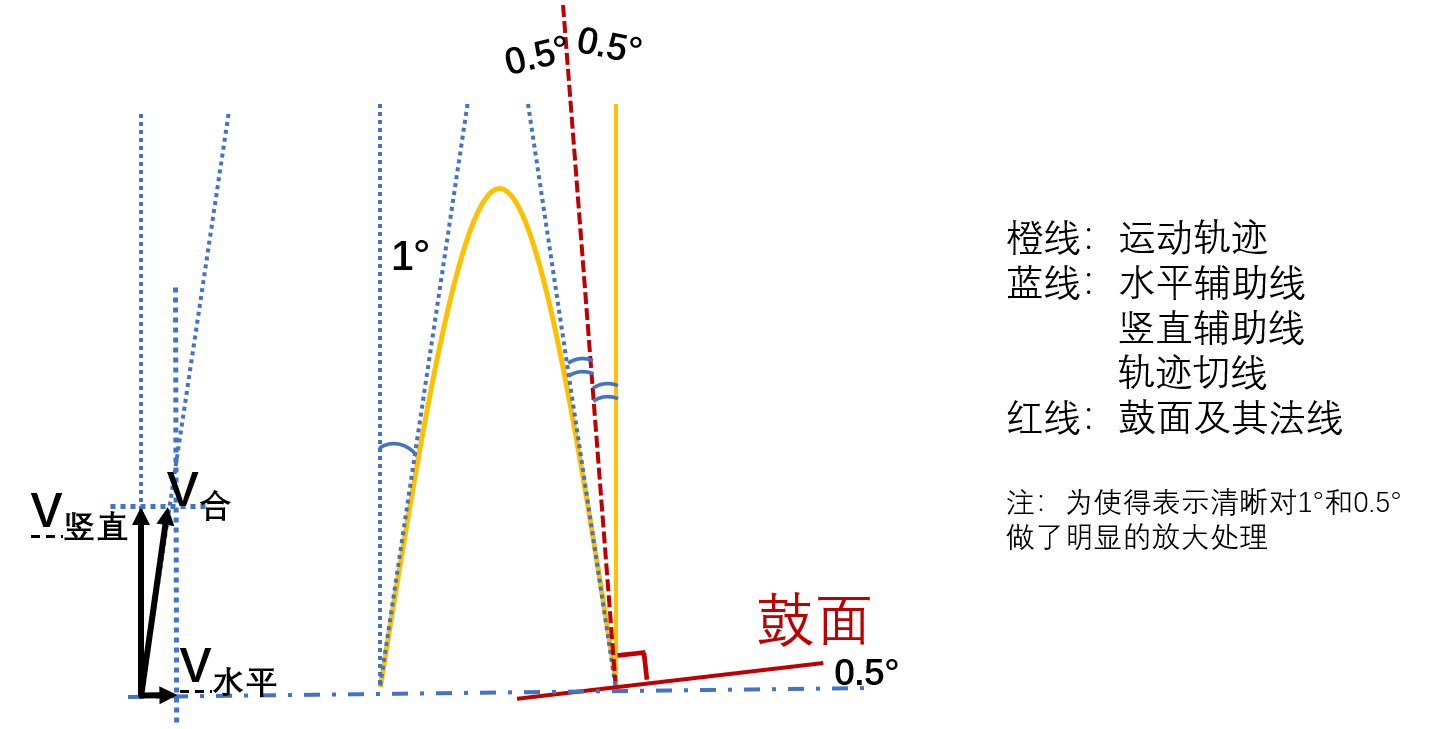
\includegraphics[width=0.8\textwidth]{figure7.png}\\ 
    图11:排球运动轨迹分析  
\end{center}
如图所示,根据镜面反射的思路,想要使得排球回到竖直弹跳状态,则鼓面需要产生与水平面0.5°的倾角。
下先就排球的运动过程进行计算与分析,再就鼓面变化所需及人的运动过程进行分析。

\subsection{问题求解}
\subsubsection{排球运动过程}
对排球运动过程分为两个部分,第一部分为斜抛过程,第二部分为碰撞过程,碰撞过程仍分为三阶段,与第一问相同。\\

\centerline{斜抛过程}

\begin{equation}
    \begin{cases}
        \frac{1}{2}gt^2=0.6\\
        v_{\mbox{竖直}}=gt\\
        v_{\mbox{合}}=\frac{v_{\mbox{竖直}}}{sin89°}\\
        v_{\mbox{水平}}=v_{\mbox{合}}cos89°\\
        x_{\mbox{水平}}=2v_{\mbox{水平}}t
    \end{cases}
\end{equation}

求解得到$x_{\mbox{水平}}=0.04189215583(m)$,$v_{\mbox{合}}=3.431557472143(m/s)$

通过第一问的讨论我们知道,若想排球与鼓面最大高度差达到40cm,并在此时求解v1的最小值,我们可以列出以下关系式

对于碰撞后鼓可能产生的竖直上抛追逐排球过程:

其中$t_1$为排球上升0.4m所需的时间,$v_0$为排球上升了0.4m后的速度,$t_2$为鼓下降到最低点所需总时间
\begin{equation}
    \begin{cases}
        v_2^{\mbox{'2}}-v_0^2=2g(0.4)\\
        t_1=\frac{ v_2^{\mbox{'}}-v_0}{g}\\
        t_2=\frac{2v_1^{\mbox{'}}}{g}\\
        t_1\ge t_2
    \end{cases}
\end{equation}

解得$ v_2^{\mbox{'}}-v_0\ge 2v_1^{\mbox{'}}$
\begin{center}
    $min \{ v_1 \}$    
\end{center}
\begin{equation}
    \begin{cases}
        v_{\mbox{合}}=3.431557472143(m/s)\\
        v_2=-v_{\mbox{合}}\\
        v_1^{\mbox{'}}=v_1-(1+e)(v_1-v_2)\frac{m_2}{m_1+m_2}\\
        v_2^{\mbox{'}}=v_2+(1+e)(v_1-v_2)\frac{m_1}{m_1+m_2}\\
        v_0^2=v_2^{\mbox{'2}}-2g(0.4)\\
        v_2^{\mbox{'}}\ge\sqrt(0.8g)\\
        v_2^{\mbox{'}}-v_0\ge 2v_1^{\mbox{'}}\\
        g=9.81; e=0.86; \\
        m1=3.6; m2=0.27;\\
    \end{cases}
\end{equation}

使用Lingo进行非线性最优化运算

\begin{center}
    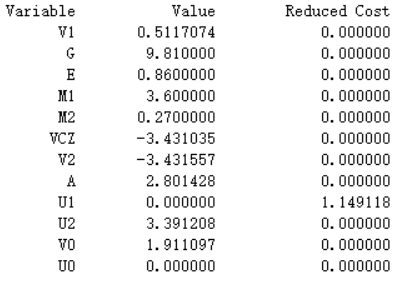
\includegraphics[width=0.5\textwidth]{figure8.png}\\ 
    图12:第一次Lingo最优运算
\end{center}

此时解出$v_1最小为0.5117074m/s$,这保证了鼓一定会有竖直上抛过程,而$v_2^{\mbox{'}}=3.3912m/s$,在如此大的反弹速度下,排球可以上升至58cm左右,远大于所需要的40cm。
故而可知,鼓不需要这么大的初速度,也即是鼓碰撞后不会发生任何上抛行为,碰后的速度可以向下。删除约束条件$v_2^{\mbox{'}}-v_0\ge 2v_1^{\mbox{'}}$重新进行最优化非线性规划。

\begin{center}
    $min \{ v_1 \}$    
\end{center}
\begin{equation}
    \begin{cases}
        v_{\mbox{合}}=3.431557472143(m/s)\\
        v_2=-v_{\mbox{合}}\\
        v_1^{\mbox{'}}=v_1-(1+e)(v_1-v_2)\frac{m_2}{m_1+m_2}\\
        v_2^{\mbox{'}}=v_2+(1+e)(v_1-v_2)\frac{m_1}{m_1+m_2}\\
        v_2^{\mbox{'}}\ge\sqrt(0.8g)\\
        g=9.81; e=0.86; \\
        m1=3.6; m2=0.27;\\
    \end{cases}
\end{equation}
使用Lingo进行非线性最优化运算的结果如图所示

\begin{center}
    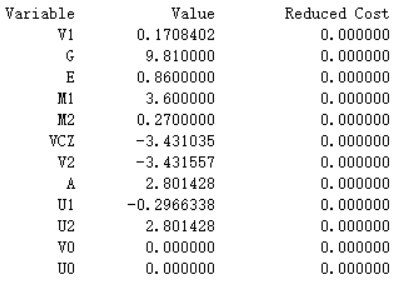
\includegraphics[width=0.5\textwidth]{figure9.png}\\ 
    图13:第二次Lingo最优运算
\end{center}

到此,我们解出,鼓被瞬时加速到的初速度只需要有0.1708402m/s即可满足条件。\\

\centerline{人拉绳的力度分析}

在鼓被瞬时加速到的初速度只需要有0.1708402m/s的条件下同第一题分析,若鼓不需偏转的话,每个人所要给出的的平均的力。
假设鼓面初始时刻是水平静止的,初始位置较绳子水平时下降11cm。

\begin{center}
    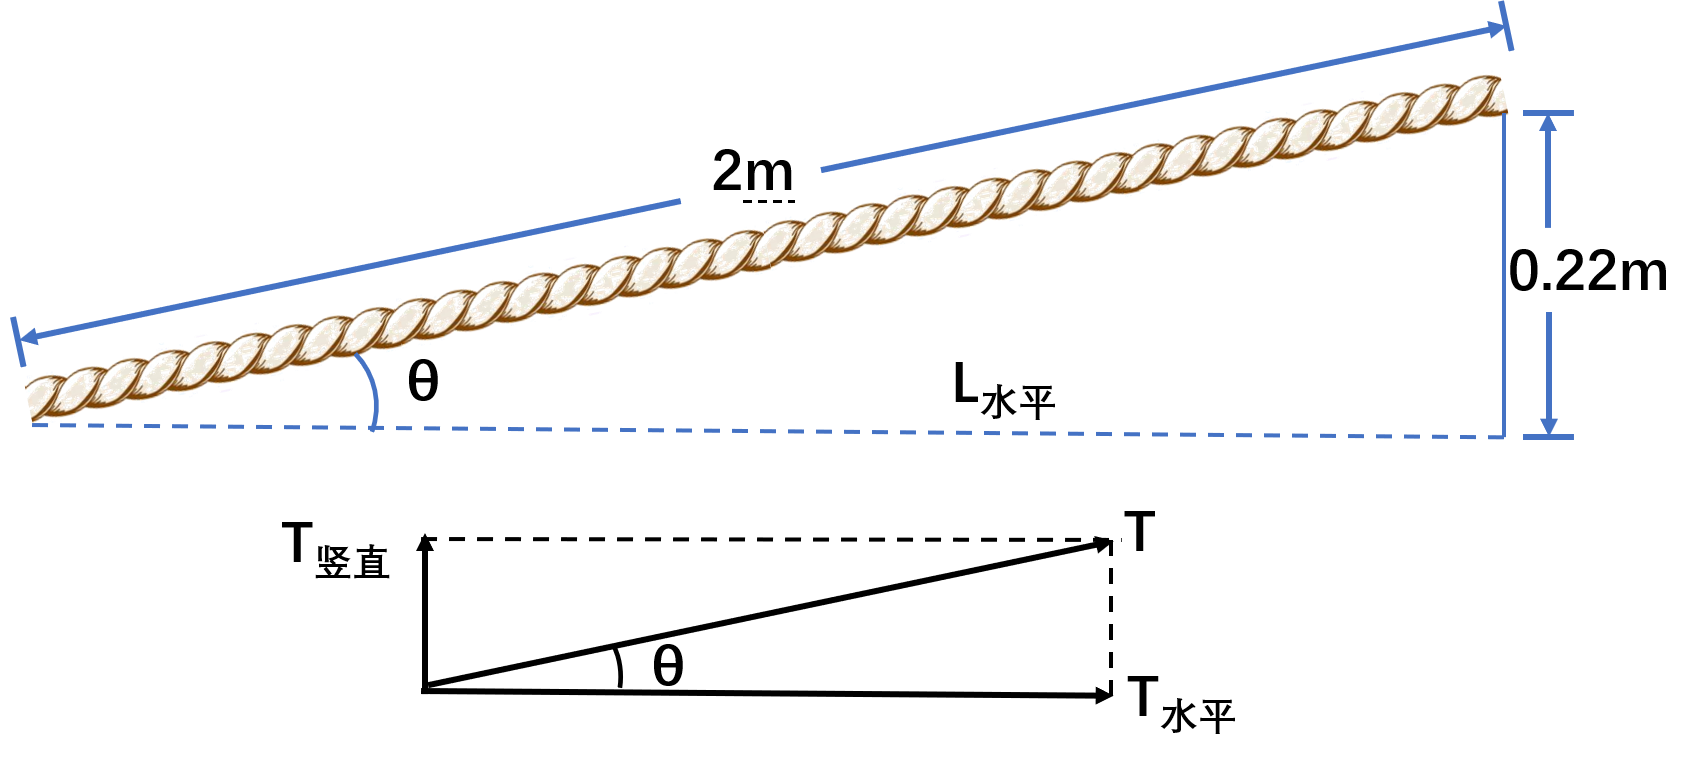
\includegraphics[width=0.6\textwidth]{figure10.png}\\ 
    图14:鼓不发生偏转时的受力分析
\end{center}

鼓是在瞬时获得的速度,鼓需要获得的瞬时冲量,此处我们仍取瞬时为0.1s
\begin{equation}
    I_1=(F_{\mbox{合竖直}}-m_1g)t_{\mbox{瞬}}=P_1=m_1v_1
\end{equation}
解得$I_1$=0.61502472(N·s)

又因为有10人拉鼓,则
\begin{equation}
    \begin{cases}
        I_1=(F_{\mbox{合竖直}}-m_1g)t_{\mbox{瞬}}\\
        t_{\mbox{瞬}}=0.1\\
        F_{\mbox{合竖直}}=10T_{\mbox{竖直}}\\
        T_{\mbox{竖直}}=sin\theta T\\
        sin\theta=\frac{11}{200}
    \end{cases}
\end{equation}

在此基础上解得T=75.39317672‬N,故而若鼓不需偏转的话,每个人所要给出的的平均的力为75.39317672N
但此时我们需要调整已偏转的鼓面,使得球在下次撞击后恢复竖直弹跳。

依图及题意易知,此时鼓偏转0.5°,要满足要求,需要使其沿当前偏转方向反向偏转1°,此时可以使用问题二模型进行求解。

题中所提夹角比1:2的队员分别为1、10号。如下图所示:
\begin{center}
    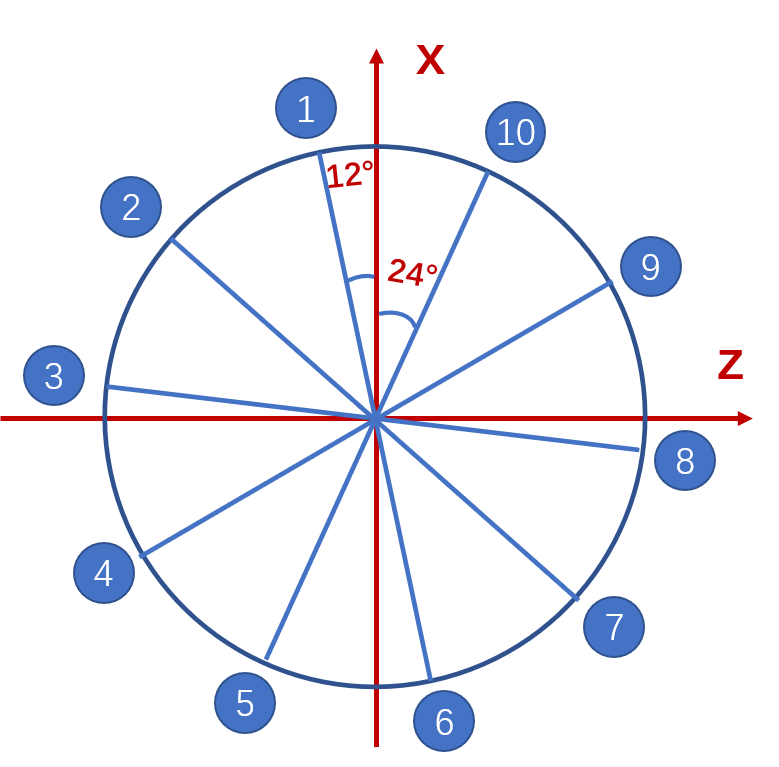
\includegraphics[width=0.5\textwidth]{figure16.png}\\ 
    图15:队员站位与坐标系
\end{center}

在所有人发力前,鼓在空中竖直方向上需受力平衡,根据题设、受力分析,解得每人应当提供64.2N的力。

我们假设每人发力的时间维持0.1s,使用二分法及微元法,经matlab求解得,1号需沿绳发力42.95806060N,10号需沿绳发力 84.03864783N,为了使得发力状态对称,需要让3号队员额外发力12.747N,即共发力76.947N,使得合力在水平面上的方向与x轴同向,其余人提供64.2N的力即可。

结合以上,1、10、3号分别沿绳给出的平均的力为54.15123732N、95.23182455N、88.14017672N

\begin{center}
    \section{模型优缺点分析及模型改进}    
\end{center}
\subsection{模型优点}
(1)问题一中我们进行了分段运动学分析,进行了精确的运动描述,对各种可能的运动状态进行了先验的预判,有利于在优化目标的过程中合理而完备的添加约束条件,使得结果的可信度提高。

(2)问题二利用刚体力学对鼓面的受力过程进行了完善、严谨、合理的分析,合理的建立坐标系,使得模型适用性极为广泛,适用于多种运动状态及角度下的鼓,
通过代入不同的位矢,可直接应用于本题后三问,结果利用微元法求解,计算简便。

(3)利用二分法及微元法,避免了求解常微分方程的难点,模型求解速度快,效率高,精度高。

(4)第三问中,通过修改发力参数和队员占位,尽可能降低失误率(即降低鼓面倾角),我们灵活的运用了第二问得到的Matlab代码。求解各种更改后所得的鼓面倾角,
对我们建立的模型进行了合理有效的验证。

(5)第四问中,我们将队员发力拆解为两部分分别进行撞击和旋转。独立的求解力的作用效果后,再进行合理的叠加,优化了解决问题的方式。通过精确的力学分析,
调整看似不相关的队员的发力情况,以使得水平受力状态不对称的系统,变得对称而可解。


\subsection{模型缺点}
(1)问题一中我们没有对瞬时形成冲量的过程进行分析,可能存在理想化问题。同时鼓面低于绳拉直平面的距离为定值,
并未将其代入非线性优化模型进行优化。这一因素的忽略可能造成误差。

(2)问题二中,对于两次时间段中,不同发力因素下,由两个角度合并为最终结果的过程比较简单。

(3)问题三中,为消除自由度,将偏转1.118°的碰撞忽略处理为对心碰撞可能对结果造成一定的影响。

(4)问题二、四当前所使用的微元步数为1000,精度并不够高。

(5)问题四中使用二分法,进行结果求解,得到的发力情况只是可行解,但并非全局最优解。

\subsection{模型改进}
(1)对于问题一,将更多的自由度纳入考虑范围,例如精确测定恢复系数,允许鼓从不同起始高度接受运动等等,来使得模型获得优化,更加贴近真实情况。

(2)问题二、四求解时,微元步长可以设置的更小,以提高求解的精度。

(3)问题三,精确的考量非对心非完全弹性碰撞的碰撞结果,对碰撞后排球速度的变化有更加精细的把握。可以使得拟合结果更加真实。

(4)求解第四题时,为了获得最优结果,需要设置一些约束条件,通过神经网络或遗传算法,求取最优化的发力方式。

\newpage
\begin{center}
    \LARGE{参考文献}    
\end{center}

\begin{thebibliography}{99}
    \bibitem{1}
    维基百科 各材料的恢复系数[DB/OL] $https://en.wikipedia.org/wiki/Coefficient_of_restitution#Range_of_values_$\\
    $for_e_.E2.80.93_treated_as_a_constant$
    \bibitem{2}
    武际可. 能量守恒定律的发现——力学史杂谈之二十[J]. 力学与实践, 2009, 31(2):99-104.
    \bibitem{3}
    段一士, 王友棠. 广义相对论中的能量动量守恒定律[J]. 物理学报, 1963, 19(11):689-704.
    \bibitem{4}
    黄海燕. 碰撞问题的能量分析[J]. 河北北方学院学报(自然科学版), 2002(4):27-29.
    \bibitem{5}
    车晓芳. 几种规则刚体转动惯量计算的探讨[J]. 牡丹江教育学院学报, 2010(6):115-116.
    \bibitem{6}
    孙克恕. 关于刚体定轴转动定律与角动量[J]. 安庆师范学院学报(自科版), 1995(2).
    \bibitem{7}
    吴其晔. 关于刚体定轴转动定律[J]. 大学物理, 1983, 1(5):5-6.
    \bibitem{8}
    李传新. 左手定则,右手定则与右手螺旋定则[J]. 荆楚理工学院学报, 2000(3):40-43.
\end{thebibliography}

\newpage
\begin{appendices}
\centerline{{\LARGE\bfseries 附录}}
%\appendixpage

\centerline{\zihao{5}\songti\thesection {附录1 \quad matlab\_2\_1.m 求解第二题第一种情况偏转角度的示例matlab代码}}
    \begin{verbatim}
        m=3.6;g=9.81;   %鼓质量、重力加速度
        Moi=0.0832057;  %转动惯量
        Ft=[90,80,80,80,80,80,80,80];  %本次发力参数,
        mass=[0,0,0];   %质心初始位置
        cord_length=1.7;   %绳长
        drop=0.11;  %鼓面距绳水平高度
        distance=radius+sqrt(cord_length^2-drop^2); %队员握绳处距质心处水平距离
        R1=[    %为便于计算,发力状态对称于xoy平面,所以根据不同的发力参数,需要确定不同的R1,为手握绳处到原点的矢量
            distance,0,drop;
            distance/sqrt(2),distance/sqrt(2),drop;
            0,distance,drop;
            -distance/sqrt(2),distance/sqrt(2),drop;
            -distance,0,drop;
            -distance/sqrt(2),-distance/sqrt(2),drop;
            0,-distance,drop;
            distance/sqrt(2),-distance/sqrt(2),drop;
            ];
        j=0.2/sqrt(2);
        y=0;   %初始旋转角度
        omega=0;   %初始角速度
        vgu=[0,0,0]; %鼓在受力过程中的速度
        for t=0:1:1000
            R2=[ %鼓边各点到质心初始位矢
            0.2,0,0.2*sin(y);
            j,j,j*sin(y);
            0,0.2,0;
            -j,j,-j*sin(y);
            -0.2,0,-0.2*sin(y);
            -j,-j,-j*sin(y);
            0,-0.2,0;
            j,-j,j*sin(y);];
        
            m=[cos(y),1,1];
            L=R2.*m; %旋转y弧度情况下,鼓边各点到质心位矢
            r=L+mass;%鼓边各点相对原点位矢
            direction=(R1-r)./sum(abs(R1-r).^2,2).^(1/2);
            F=Ft'.*direction;
            
            z=cross(F,L);
            c=sum(z);
            A=c/Moi;
            u=A(2);
        
            Fs=sum(F);
            agu=Fs./3.6;
            agu(3)=agu(3)-g;
            mass=mass+vgu*0.0001+agu.*(0.0001)^2/2;
            vgu=vgu+agu*0.0001;
            
            m=omega*0.0001+u*(0.0001)^2/2;
            omega=omega+u*0.0001;
            y=y+m;
        end
        y=y*180/pi
      
    \end{verbatim}

\centerline{\thesection {附录2 \quad matlab\_2\_2.m 求解第二题第二种情况偏转角度的示例matlab代码}}
 \begin{verbatim}
            m=3.6;
            g=9.81;
            Moi=0.0832057;
            Ft=[90,90,80,80,80,80,80,80];
            mass=[0,0,0];
            radius=0.2;
            cord_length=1.7;
            drop=0.11;
            distance=radius+sqrt(cord_length^2-drop^2);
            cosd=cos(22.5*pi/180);
            sind=sin(22.5*pi/180);
            R1=[
                distance*cosd,-distance*sind,drop;
                distance*cosd,distance*sind,drop;
                distance*sind,distance*cosd,drop;
                -distance*sind,distance*cosd,drop;
                -distance*cosd,distance*sind,drop;
                -distance*cosd,-distance*sind,drop;
                -distance*sind,-distance*cosd,drop;
                distance*sind,-distance*cosd,drop;
                ];
            j=0.2/sqrt(2);
            y=0;
            v=0;
            vgu=0;
            for t=0:1:1000
                R2=[
                0.2*cosd,-0.2*sind,0.2*sin(y);
                0.2*cosd,0.2*sind,0.2*sin(y);
                0.2*sind,0.2*cosd,0;
                -0.2*sind,0.2*cosd,-0.2*sin(y);
                -0.2*cosd,0.2*sind,-0.2*sin(y);
                -0.2*cosd,-0.2*sind,-0.2*sin(y);
                -0.2*sind,-0.2*cosd,0;
                0.2*sind,-0.2*cosd,0.2*sin(y);];
            
                m=[cos(y),1,1];
                L=R2.*m;
                r=L+mass;
                direction=(R1-r)./sum(abs(R1-r).^2,2).^(1/2);
                F=Ft'.*direction;
                
                z=cross(F,L);
                c=sum(z);
                A=c/Moi;
                u=A(2);
                
                Fs=sum(F);
                agu=Fs./3.6;
                agu(3)=agu(3)-g;
                mass=mass+vgu*0.0001+agu.*(0.0001)^2/2;
                vgu=vgu+agu*0.0001;
                
                m=v*0.0001+u*(0.0001)^2/2;
                v=v+u*0.0001;
                y=y+m;
            end
            y=y*180/pi
            
            
            %3的Ft、R1、R2如下,其余按思路,基本都可由已有的1、2、3代码更改F或R1或R2推出,其余人在未发力时,力的大小经受力平衡计算,为68.2左右
            %3:
            % cosd=cos(22.5*pi/180);
            % sind=sin(22.5*pi/180);
            % Ft=[90,80,80,90,80,80,80,80];
            % R1=[
            %     distance*sind,-distance*cosd,drop;
            %     distance*cosd,-distance*sind,drop;
            %     distance*cosd,distance*sind,drop;
            %     distance*sind,distance*cosd,drop;
            %     -distance*sind,distance*cosd,drop;
            %     -distance*cosd,distance*sind,drop;
            %      -distance*cosd,-distance*sind,drop;
            %     -distance*sind,-distance*cosd,drop; 
            %     ]
            % R2=[
            %     0.2*sind,-0.2*cosd,0.2*sin(y);
            %     0.2*cosd,-0.2*sind,0.2*sin(y);
            %     0.2*cosd,0.2*sind,0.2*sin(y);
            %     0.2*sind,0.2*cosd,0;
            %     -0.2*sind,0.2*cosd,-0.2*sin(y);
            %     -0.2*cosd,0.2*sind,-0.2*sin(y);
            %     -0.2*cosd,-0.2*sind,-0.2*sin(y);
            %     -0.2*sind,-0.2*cosd,0;
            %    ]
  
\end{verbatim}

\centerline{\thesection {附录3 \quad matlab\_4\_1.m 求解第四题中获取偏转角度所需力的matlab代码}}
 \begin{verbatim}
            m=3.6;g=9.81;   %鼓质量、重力大小
        Moi=0.0832057;  %转动惯量
        k=sin(24*pi/180)/sin(12*pi/180)
        cord_length=2;   %绳子长度
        drop=0.11;  %相较绳子水平时下落高度
        distance=radius+sqrt(cord_length^2-drop^2) %队员们手握绳子处与原点的水平距离
        step=12:36:360
        step=step*pi/180
        R1=[    %坐标系中,各个队员手握绳子处坐标,为简化模型、方便计算,此坐标下,发力状态以x、z轴平面对称
            distance*cos(step(10)),distance*sin(step(10)),0.11;
            distance*cos(step(1)),distance*sin(step(1)),0.11;
        distance*cos(step(2)),distance*sin(step(2)),0.11;
            distance*cos(step(3)),distance*sin(step(3)),0.11;
            distance*cos(step(4)),distance*sin(step(4)),0.11;
            distance*cos(step(5)),distance*sin(step(5)),0.11;
            distance*cos(step(6)),distance*sin(step(6)),0.11;
            distance*cos(step(7)),distance*sin(step(7)),0.11;
            distance*cos(step(8)),distance*sin(step(8)),0.11;
            distance*cos(step(9)),distance*sin(step(9)),0.11;
            ]

        Fmax=100;
        Fmin=21.72;%因鼓存在重力,经计算得到的最小值。
        dF=Fmax-Fmin;
        while(dF>0.001)
            y=-0.5*pi/180;
            omega=0;   %向上运动的速度
            vgu=0;
            mass=[0,0,0];
            Fc=(Fmax+Fmin)/2
            Ft=[Fc,k*Fc,64.2,64.2+12.747,64.2,64.2,64.2,64.2,64.2,64.2];
            for t=0:1:1000
                R2=[
                0.2*cos(step(10)),0.2*sin(step(10)),0.2*cos(step(10))*sin(y);
                0.2*cos(step(1)),0.2*sin(step(1)),0.2*cos(step(1))*sin(y);
                0.2*cos(step(2)),0.2*sin(step(2)),0.2*cos(step(2))*sin(y);
                0.2*cos(step(3)),0.2*sin(step(3)),0.2*cos(step(3))*sin(y);
                0.2*cos(step(4)),0.2*sin(step(4)),0.2*cos(step(4))*sin(y);
                0.2*cos(step(5)),0.2*sin(step(5)),0.2*cos(step(5))*sin(y);
                0.2*cos(step(6)),0.2*sin(step(6)),0.2*cos(step(6))*sin(y);
                0.2*cos(step(7)),0.2*sin(step(8)),0.2*cos(step(7))*sin(y);
                0.2*cos(step(8)),0.2*sin(step(8)),0.2*cos(step(8))*sin(y);
                0.2*cos(step(9)),0.2*sin(step(9)),0.2*cos(step(9))*sin(y);];

                m=[cos(y),1,1];
                L=R2.*m;
                r=L+mass;
                direction=(R1-r)./sum(abs(R1-r).^2,2).^(1/2);
                F=Ft'.*direction;
                z=cross(F,L);
                c=sum(z);
                A=c/Moi;
                u=A(2);
            
                Fs=sum(F);
                agu=Fs./3.6;
                agu(3)=agu(3)-g;
                mass=mass+vgu*0.0001+agu.*(0.0001)^2/2;
                vgu=vgu+agu*0.0001;
            
                m=omega*0.0001+u*(0.0001)^2/2;
                omega=omega+u*0.0001;
                y=y+m;
            end
        y=y*180/pi;
        if y>0.5
            Fmax=Fc;
        else
            Fmin=Fc;
        end
        dF=Fmax-Fmin;
        end
        Fc;
        k*Fc;
\end{verbatim}

\centerline{\thesection {附录4 \quad 1-1.lg4 求解第一题总功最小的非线性规划Lingo代码}}
 \begin{verbatim}
    min= 1/2*m1*v1^2+m1*g*h1;

    h1+h2=0.4;
    v2+@sqrt(2*g*h2)=0;
    u1-v1+(1+e)*(v1-v2)*m2/(m1+m2)=0;
    u2-v2-(1+e)*(v1-v2)*m1/(m1+m2)=0;
    u2+v2>=0;
    u2^2-2*u2*u1-2*h2*g>=0;
    
    g=9.81;
    e=0.86;
    m1=3.6;
    m2=0.27;
    @free(v2);
\end{verbatim}

\centerline{\thesection {附录5 \quad 4-1.lg4 求解第四题鼓速度最小的非线性规划Lingo代码}}
 \begin{verbatim}
    min=v1;

    g=9.81;
    e=0.86;
    m1=3.6;
    m2=0.27;
    vcz=-@sqrt(1.2*g);
    v2=vcz/0.99984769515639;
    a=@sqrt(0.8*g);
    u1=v1-(1+e)*(v1-v2)*m2/(m1+m2);
    u2=v2+(1+e)*(v1-v2)*m1/(m1+m2);
    v0^2=u2^2-0.8*g;
    u2>=a;
    u2-u0>=2*u1;
    
    @free(v2);
    @free(vcz);
\end{verbatim}

\centerline{\thesection {附录6 \quad 4-2.lg4 求解第一题鼓速度最小的非线性规划Lingo代码}}
 \begin{verbatim}
    min=v1;

    g=9.81;
    e=0.86;
    m1=3.6;
    m2=0.27;
    vcz=-@sqrt(1.2*g);
    v2=vcz/0.99984769515639;
    a=@sqrt(0.8*g);
    u1=v1-(1+e)*(v1-v2)*m2/(m1+m2);
    u2=v2+(1+e)*(v1-v2)*m1/(m1+m2);
    v0^2=u2^2-0.8*g;
    u2>=a;
    
    @free(v2);
    @free(vcz);
    @free(u1);
\end{verbatim}

\centerline{\thesection {附录7 \quad 绳长.py 求解第一题最短绳长的Python代码}}
 \begin{verbatim}
    from math import *

    L=0.6*sqrt(2+sqrt(2))/sqrt(2)
    
    a=sqrt(L*L+0.31*0.31)
    
    sin=0.31/a
    
    print('L=',L)
    print('a=',a)
    print('sin=',sin)
\end{verbatim}
\end{appendices}

\end{document}
